\documentclass[11pt,a4paper]{article}

\usepackage[margin=1in, paperwidth=8.3in, paperheight=11.7in]{geometry}
\usepackage{amsmath,amsfonts,bbm,caption,changepage,fancyhdr,graphicx,tikz,subcaption}
\usetikzlibrary{automata,positioning}
\graphicspath{ {img/} }
\usepackage[section,nohyphen]{DomH}
\headertitle{IEFT - Reviewed Notes}

\begin{document}

\title{Internet Economics and Financial Technology - Reviewed Notes}
\author{Dom Hutchinson}
\date{\today}
\maketitle

\tableofcontents\newpage

\section{Economic Theory} \label{sec_EconomicTheory}

\subsection{General} \label{sec_GeneralEconomicTheory}

  \begin{definition}{Economic Agent}
    An \textit{Economic Agent} is someone who interacts with an economic market. \textit{Economic Agents} are typically split into two categories
    \begin{itemize}
      \item \textit{Producers} - Those making products which are then sold.
      \item \textit{Consumers} - Those who buy the products.
    \end{itemize}
    In practice most people fulfil both roles (e.g. factories sell products but buy raw materials) but not in the same market.
  \end{definition}

  \begin{definition}{Externality}
    An \textit{Externality} is a cost of benefit caused by the production or consumption of a good which is not financial (e.g. Pollution is a negative externality).
  \end{definition}

  \begin{definition}{Monopolised Markets}
    A market is \textit{Monopolised} if it is dominated by a single seller. In a \textit{Monopolised} market the \textit{Monopolising} faces little, or no, competition and thus can be \textit{price setters}, rather than price takers.
    \par IRL a firm with over $40\%$ market share is considered to have a monopoly.
  \end{definition}

  \begin{remark}{Experimental Economics - Human Trading Behaviours}
    \textit{Experimental Economics} is a field of Economics where lab-style studies are used to study economic questions.
    \par In this unit we are interested in how \textit{Experimental Economics} approaches the study of human trading behaviours. The general approach is the following
    \begin{itemize}
      \item Have a small number of human subjects split into ``buyers'' and ``sellers''.
      \item Assign each subject a private-value/limit price which they are not allowed to exceed.
      \item Provide subjects with a market to interact with where they can post prices.
      \item Observe the subjects behaviours under different market conditions.
    \end{itemize}
  \end{remark}

  \begin{proposition}{Experiment Design}

  \end{proposition}

\subsection{Micro-Economics} \label{sec_MicroEconomics}

  \begin{definition}{Micro-Economics}
      \textit{Micro-Economics} is the study of the behaviour of individual economic agents (e.g. individuals or businesses) in the allocation and making of limited resources. Typically these agents are partitioned into consumers and producers.
      \par This can be considered as the study of \textit{Supply-and-Demand}.
  \end{definition}

  \begin{remark}{Effect of Scarcity}
    Producers have a limited number of resources which they can convert into products and consumers have a limited amount of money with which to purchase goods. This means there are prices which are too low for a producer to be willing to sell at, and prices which are too high for a consumer to be willing to purchase at.
  \end{remark}

  \begin{definition}{Production Costs}
    The cost incurred by a producer to produce a product can be split into three categories. These categories aim to explain how costs are effected by quantity produced.
    \begin{itemize}
      \item \textit{Fixed Costs} - Costs a producer incurs regardless of amount produced (e.g. rent).
      \item \textit{Variable Costs} - Costs which depend on quantity being produced (e.g. raw materials).
      \item \textit{Semi-Variable Costs} - Costs which in part stay consistent and in part vary with quantity produced (e.g. commissions in wages).
    \end{itemize}
  \end{definition}

  \begin{remark}{Production Costs}
    These categories are very idealised. \textit{Fixed Costs} do actually increase when the quantity produced increases (e.g. needing to rent a large factory) but at a much slower (and likely stepped) fashion that \textit{Variable Costs}.
  \end{remark}

  \begin{definition}{Net Utility}
    \textit{Net Utility} for a product is the difference between the price a consumer pays for it and the perceived value they have for the product. This is similar to \textit{Consumer Excess} and consumers want to maximise their \textit{Net Utility}.
  \end{definition}

\subsubsection{Supply-and-Demand Curve} \label{sec_SupplyAndDemandCurve}

  \begin{figure}[ht!]
    \centering
    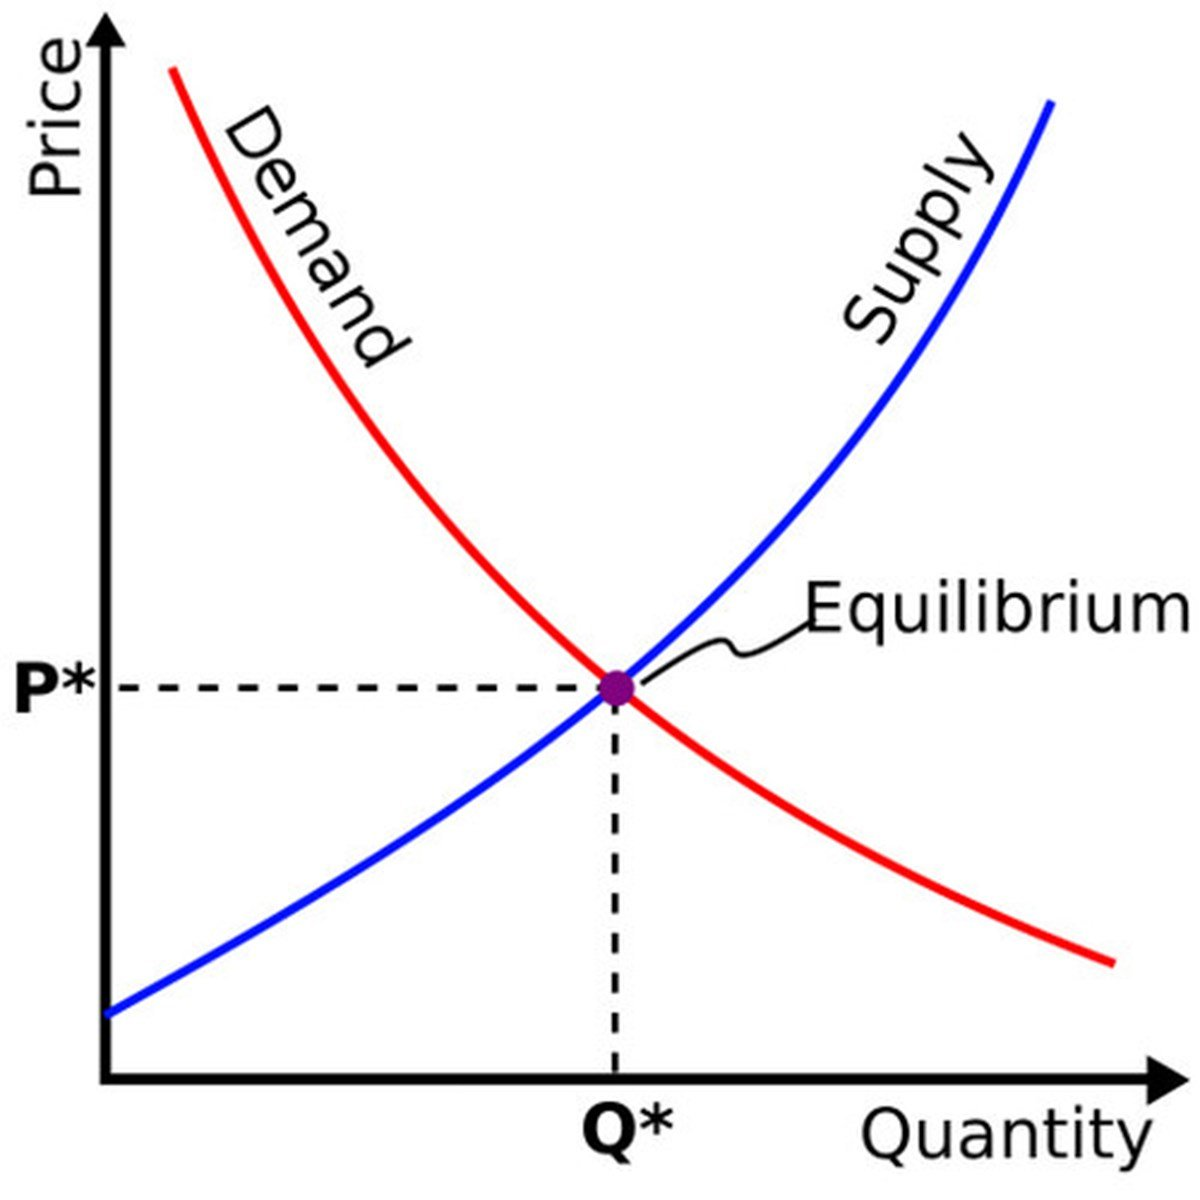
\includegraphics[width=.3\textwidth]{SupplyAndDemandCurve.jpg}
    \caption{Example of Market Supply-and-Demand Curves}
    \label{fig_SupplyAndDemandCurve}
  \end{figure}

  \begin{definition}{Supply-and-Demand Curve}
    \textit{Supply-and-Demand Curves} are plots of price-per-unit against quantity, and summarise the price per unit agents in a market (consumers and producers) are willing to accept for different quantities of a product.
    % Consumer Demand Curve
    \par A \textit{Market Demand Curve} shows the total quantity of a product which all consumers in a market would buy at different price points. A \textit{Demand Curve} slopes down as it is assumed that consumers are always willing to accept to a lower price-per-unit but not necessarily a higher price.
    % Market Supply Curve
    \par A \textit{Market Supply Curve} shows the total quantity of products all producers in a market would produce if they were to receive certain prices. A \textit{Supply Curve} slopes upwards as it is assumed that producers will always accept a higher price, but not necessarily a lower price.
    \par See \texttt{Figure 1.\ref{fig_SupplyAndDemandCurve}} for an example of these curves.
  \end{definition}

  \begin{definition}{Business Supply Curve}
    A \textit{Business Supply Curve} is similar to a \textit{Market Supply Curve} except it is only concerned with a single business in the market. The \textit{Business Supply Curve} plots the minimum price-per-unit a business is willing to accept for different quantities of goods sold. Generally this tracks the marginal cost of producing the goods at these quantities.
    \par \textit{Business Supply Curves} tend to be truncated as there are quantities which are too small for a business to deem them feasible at all.
  \end{definition}

  \begin{remark}{Shifting Supply-and-Demand Curves}
    Supply-and-Demand Curves can \textit{Shift}. These \textit{Shifts} occur due to non-price factors such as a pandemic, or improvements in the production process. A \textit{Shift} will cause a movement in the \textit{Market Equilibrium.}
  \end{remark}

  \begin{figure}[ht!]
    \centering
    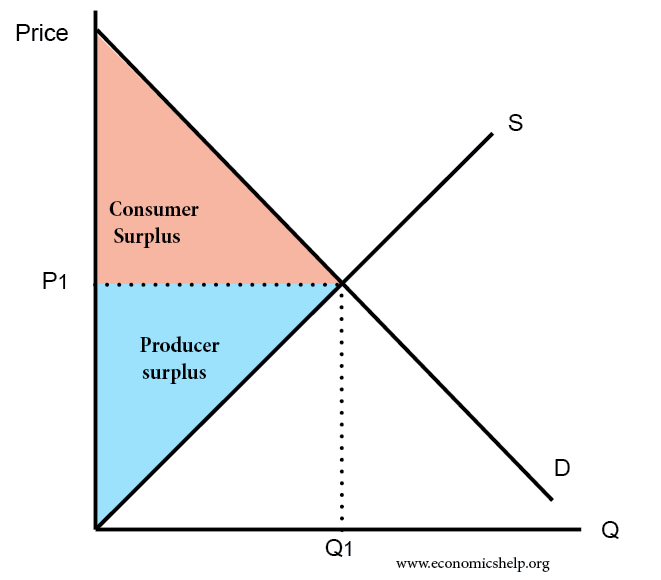
\includegraphics[width=.3\textwidth]{Surplus.PNG}
    \caption{Illustration of excess for given prices}
    \label{fig_SupplyAndDemandSurplus}
  \end{figure}

  \begin{definition}{Surplus}
    \textit{Surplus} is the difference between the price an agent was willing to accept and the price they actually accepted (ie the market price). All agents was to maximise their surplus (ie Producers want as high a price as possible \& Consumers want as low a price as possible).
  \end{definition}

  \begin{definition}{Equilibrium}
    A competitive market the \textit{Market Equilibrium} is the price at which the quantity demanded and quantity supplied by a market is equal (ie the intersection of supply and demand curves). This is the price at which \textit{Surplus} is maximised for both consumers and producers.
    \par This can be seen in a \textit{Supply-Demand Graph} as the point where hte supply and demand curves intersect.
  \end{definition}

  \begin{remark}{Dynamic Variation of Equilibrium}
    In reality \textit{Market Equilibria} are dynamic as consumers and producers often leave the market after completing a transaction. This is more apparent in small markets.
  \end{remark}

  \begin{definition}{Pareto Efficient Allocation}
    An allocation of resources is \textit{Pareto Efficient} if any change to the allocation would definitely end up with someone being worse off.
  \end{definition}

\subsubsection{Economies of Scale} \label{sec_EconomiesOfScale}

  \begin{figure}[ht!]
    \centering
    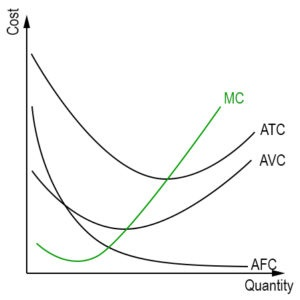
\includegraphics[width=.3\textwidth]{MarginalCostCurve.jpg}
    \caption{Illustration of typical relationship between quantity produced and: Marginal Cost (MC); Average Total Costs (ATC); Average Variable Costs (AVC); and, Average Fixed Costs (AFC)}
    \label{fig_MarginalCostCurve}
  \end{figure}

  \begin{definition}{Marginal Cost}
    \textit{Marginal Cost} of production is the cost to produce one extra unit. This value will vary depending upon the total number of units being produced due to \textit{Economies of Scale}.
    \par \textit{Marginal Cost} combines \textit{Fixed Costs} and \textit{Variable Costs}. As the quantity of units being produced increases, average-fixed-costs-per-unit will always decrease but average-variable-costs-per-unit may increase.
    \[ \text{Marginal Cost}=\frac{\text{Change in Production Costs}}{\text{Change in Quantity Produced}} \]
  \end{definition}

  \begin{definition}{Marginal Cost Curve}
    \textit{Marginal Cost Curves} is a plot of price-per-unit against quantity, showing the marginal cost of producing extra units wrt the total number of units being produced. \textit{Marginal Cost Curves} typically have a $U$-shape.
    \par See \texttt{Figure \ref{fig_MarginalCostCurve}}.
  \end{definition}

  \begin{proposition}{Minimum Sale Price}
    \par In the short-run, for a producer to stay in business, they need the average sale price of each unit to be greater than their \textit{Average Variable Costs} (AVC).
    \par In the long-run, for a producer to say in business, they need to cover their fixed costs too. Thus, the average sale price of each unit needs to be greater than the \textit{Average Total Cost} (ATC).
    \par These two metrics provide a minimum sales price for both the short- and long-term
  \end{proposition}

  \begin{definition}{Economies of Scale}
    \textit{Economies of Scale} are production cost savings which are obtained due to scaling the quantity of products being produced. These occur where the \textit{Marginal Cost Curve} has a negative gradient (ie marginal cost is decreasing).
    \par \textit{Economies of Scale} occur, in practice, from maximising the potential of all machines/workers and bulk buying raw materials.
  \end{definition}

  \begin{remark}{Dis-Economies of Scale}
    The scale of a business can grow too large and \textit{Dis-Economies of Scale} occur. Practically this can occur due to increased logistical difficulties. \textit{Dis-Economies of Scale} are occuring when the \textit{Marginal Cost Curve} has a positive gradient (ie marginal costs are increasing).
  \end{remark}

\subsubsection{Price Elasticity} \label{sec_PriceElasticity}

  \begin{definition}{Price Elasticity}
    \textit{Price Elasticity} is a measure of how changes in price and quantity demanded/supplied affect each other. This is quantified by the inverse gradient of a supply-curve or a demand-curve. The shallower the gradient (ie flatter the curve) the greater the quantity available will change for a given change in price.
    \[ \text{PE}=\left|\frac{\text{Change in Quantity Demanded/Supplied}}{\text{Change in Price}}\right| \]
    \par There are some special cases:
    \begin{itemize}
      \item \textit{Perfect Price Elasticity} ($PE=\infty$) - A change in quantity has no affect on price. This is when the supply/demand-curve is horizontal.
      \item \textit{Perfect Price \underline{In}elasticity} ($PE=0$) - The same quantity is demanded/supplied regardless of price. This is when the supply/demand-curve is vertical.
      \item \textit{Unit Price Elasticity} ($PE=1$) - A $\Delta\%$ change in price leads to a $\Delta\%$ change in quantity demanded/supplied. This is when the supply/demand-curves are $45^o$.
    \end{itemize}
  \end{definition}

  \begin{remark}{Elastic v Inelastic}
    A product is said to \textit{Price Elastic} if $PE>1$ and \textit{Price \underline{In}elastic} if $PE<1$.
  \end{remark}

  \begin{remark}{Price Elasticity - Supply}
    The \textit{Price Elasticity} of supply quantifies how much the price of a product needs to be increased in order for the producer to be able/willing to meet the new demand.
  \end{remark}

  \begin{proposition}{Factors Affecting Elasticity of Supply}
    There are several factors which can the \textit{Price Elasticity} of producers:
    \begin{enumerate}
      \item Whether there is any spare production capacity.
      \item Current stock levels of a product. And thus, how feasible it is to store a product.
      \item How long it takes to produce the product.
      \item How easy is it to scale. If specialised workers and tools are required then prices will be more \underline{in}elastic.
    \end{enumerate}
  \end{proposition}

  \begin{proposition}{Factors Affecting Elasticity of Demand}
    There are several factors which can the \textit{Price Elasticity} of producers:
    \begin{enumerate}
      \item Necessity of the product. Luxuries will be more \textit{Price Elastic} than necessities.
      \item Availability of substitutes.
      \item Ability to postpone consumption.
      \item Relative price level (as a proportion of total expenditure).
    \end{enumerate}
  \end{proposition}

\subsubsection{Price Discrimination} \label{sec_PriceDiscrimination}

  \begin{figure}[ht!]
    \centering
    \begin{subfigure}[b]{.3\textwidth}
         \centering
         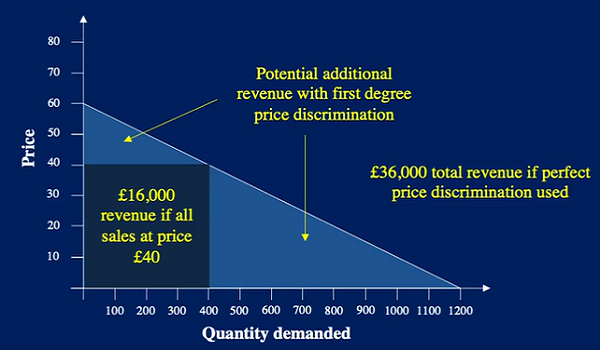
\includegraphics[width=\textwidth]{personalisedPricing.PNG}
         \caption{$1^\text{st}$ Degree}
    \end{subfigure}
    \begin{subfigure}[b]{.3\textwidth}
        \centering
        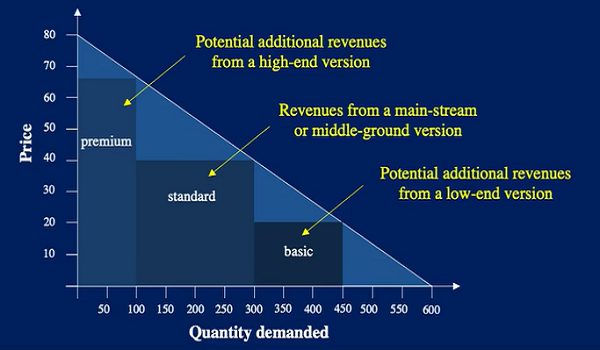
\includegraphics[width=\textwidth]{versioningPricing.PNG}
        \caption{$2^\text{nd}$ Degree}
    \end{subfigure}
    \begin{subfigure}[b]{.3\textwidth}
         \centering
         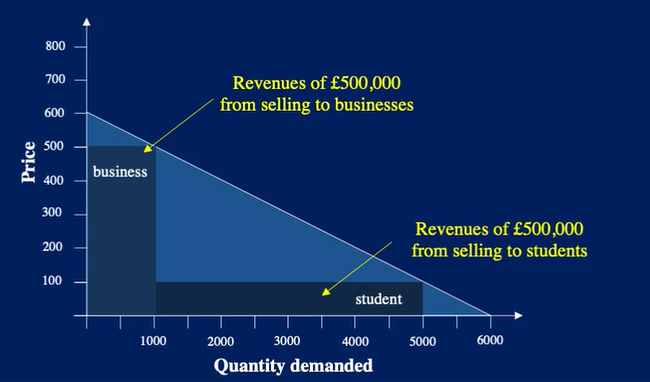
\includegraphics[width=\textwidth]{groupPricing.PNG}
         \caption{$3^\text{rd}$ Degree}
     \end{subfigure}
    \caption{Potential revenue increases for different pricing strategies}
    \label{fig_PriceDiscrimination}
  \end{figure}

  \begin{definition}{Price Discrimination}
    \textit{Price Discrimination} is the practice of charging different prices to different customers, for the same product. There are three levels of \textit{Price Discrimination}
    \begin{itemize}
      \item \textit{$1^{st}$ Degree} (Personalised Pricing) Producers charge each consumer the maximum price they are willing to pay (AKA \textit{Perfect Price Discrimination}).
      \item \textit{$2^{nd}$ Degree} (Versioning) Producers charge different prices for different quantities/qualities of a product. The consumer will pick the version which is most appealing to them.
      \item \textit{$3^{rd}$ Degree} (Group Pricing) Producers charge customers different prices depending on what group the customer falls into. Typically groups are based on age or location. Consumers do not get to pick which group they are a part of.
    \end{itemize}
  \end{definition}

  \begin{remark}{Utility of Price Discrimination}
    \textit{Price Discrimination} helps a producer to increase their revenue (improving their surplus) by setting different price points which capture more of the market. See \texttt{Figure 1.\ref{fig_PriceDiscrimination}} for a plot of how this can be achieved.
  \end{remark}

  \begin{remark}{Consumer Opinion - Personalised Pricing}
    Consumers tend to perceive personalised pricing as unfair, and typically like transparency in how prices are set.
  \end{remark}

  \begin{proposition}{When is Price Discrimination Possible}
    For a producer to be able to effectively price discriminate then must fulfil the following criteria:
    \begin{enumerate}
      \item Able to distinguish between customers in order to know what price to charge them.
      \item Resale is impractical, otherwise arbitrage is possible.
      \item Have enough market power to be able to set prices above marginal costs.
    \end{enumerate}
    Criteria i) \& ii) are much more common for online businesses, than IRL businesses.
  \end{proposition}

  \begin{proposition}{Price Discrimination in Practice}
    Here are a few techniques for implementing price discrimination.
    \begin{itemize}
      \item \textit{Loyalty Schemes} - Offer the customer a discount after buying several items, this is \textit{$2^{nd}$ Degree Price Discrimination}. Also making profiling customers easier.
      \item \textit{Price Steering} - By showing customers extremely cheap/expensive products first you can influence the price customers expect to pay, this is can achieve \textit{$1^{st}$ Degree Price Discrimination}
      \item \textit{Bundling} - Selling several goods together to encourage customers to buy more products than they otherwise would. This is \textit{$2^{nd}$ Degree Price Discrimination}. (e.g. Microsoft Office vs the individual softwares).
    \end{itemize}
  \end{proposition}

  \begin{remark}{Competing with Yourself}
    \textit{Versioning} caries a risk of competing against yourself as customer who are willing to pay a higher price may choose not to if one of your versions has the specific functionality they are seeking.
  \end{remark}

  \begin{example}{Economics of Versioning}
    Suppose we have two products: Full version $X$; and, a cutdown version $X_c$. And, suppose there are two customers $A$ \& $B$ who value our products as follows
    \begin{center}
      \begin{tabular}{|c|c|c|}
        \hline
        &$X$&$X_c$\\
        \hline
        $A$&£20&£8\\
        $B$&£8&£7\\\hline
      \end{tabular}
    \end{center}
    We assume that a customer will buy a product if they have a positive \textit{Net Utility} for it, and if they have a positive \textit{Net Utility} for both products then they will buy the one with the greater \textit{Net Utility} to them (or the better version). Consider the following pricing structures
    \begin{center}
      \begin{tabular}{|c|c|c|c|c|c|}
        \hline
        $(X,X_c)$&A's Net Utility&A's Purchase&B's Net Utiltiy&B's Purchase&Total Income\\
        \hline
        (£10,-)&(£10,-)&$X$&(-£2,-)&None&£10\\
        (£10,£5)&(£10,£3)&$X$&(-£2,£2)&$X_c$&£15\\
        (£19,£7)&(£1,£1)&$X$&(-£11,£0)&$X_c$&£26\\\hline
      \end{tabular}
    \end{center}
    The last pricing structure is actual the maximum income we can achieve in this scenario.
  \end{example}

\subsection{Auction Theory} \label{sec_AuctionTheory}

  \begin{definition}{Auction}
    \textit{Auctions} facilitate the transactions of goods by enforcing a set of rules on participants. Typically there is a single auctioneer (who ensures the rules are followed), several buyers and one/several sellers. There are several categories of \textit{Auction}
    \begin{itemize}
      \item \textit{Posted Auction} - The seller \textit{``posts''} a price which bidders have to meet (This is how most shops work).
      \item \textit{Forward Auction} - The bidders offer prices to the seller with the highest price winning. The rules of the auction define how bids are placed. (See \texttt{\ref{sec_TypesOfForwardAuction} Types of Forward Auction}).
      \item \textit{Reverse Auction} - Several sellers offer prices to a buyer with the lowest price winning. (This is typically used for construct contracts).
      \item \textit{Double Auction} - All buyers and sellers are able to lists prices and whenever a compatible pair of prices are listed a transaction occurs between those parties. (\textit{Continuous Double Auctions} are used by stock markets).
    \end{itemize}
  \end{definition}

  \begin{remark}{Utility of Auctions}
    \textit{Auctions} are allow for products to be sold at a price wholey decided by the consumer's willingness to spend (ie how much they value the product). This can be an effective method for \textit{Price Discovery}
  \end{remark}

  \begin{definition}{Private Value}
    A bidders's \textit{Private Value} is the value they place on a product in an auction. Each bidder only knows their \textit{Private Value} and this will typically be the limit of what they are willing to spend on the item.
    \par \textit{Private Values} are typically imagined as being fixed before the auction. If this is not the case then \textit{Interdependence} occurs as the bidder will change their \textit{Private Value} depending on the actions of others.
  \end{definition}

  \begin{definition}{Incentive Compatible}
    A style of auction is \textit{Incentive Compatible} if it encourages bidders to bid their true value (ie \textit{Private Value}). These auctions are popular with auctioneers. (English and SPSB auctions are \textit{Incentive Compatible}).
  \end{definition}

  \begin{theorem}{Revenue Equivalence Theorem}
    The \textit{Revenue Equivalence Theorm} states
    \begin{quote}
      If \textit{Private Values} are IID and all bidders are risk neutral, then any standard auction yields the same expected revenue for the seller.
    \end{quote}
    In practice this theorem does not hold are bidders are risk adverse and interdependence exists.
  \end{theorem}

  \begin{definition}{Signalling}
    \textit{Signalling} is the practice of bidders making bids in \textit{``weird''} ways, with the intent to signal some information to other bidders. This is a form of collusion (although within the rules of the auction) and is typically used when multiple versions of the same product are on offer, allowing all participants to pay less.
  \end{definition}

  \begin{remark}{Assumptions in Auction Theory}
    \textit{Auction Theory} makes the following assumptions (which limit its practical applications)
    \begin{itemize}
      \item All auctions are equally attractive (ie people will turn up).
      \item There is no collusion between bidders.
    \end{itemize}
  \end{remark}

\subsubsection{Types of Forward Auction} \label{sec_TypesOfForwardAuction}

\subsection*{Open Auctions}

  \begin{definition}{Open Auction}
    An \textit{Open Auction} is a \textit{Forward Auction} where bids are known to all participants. There are two main types of \textit{Open Auction}: An \textit{English Auction} (As used in \textit{Homes under the Hammer}); and, a \textit{Dutch Auction} (As used in Dutch tulip markets).
  \end{definition}

  \begin{definition}{English Auction}
    An \textit{English Auction} (AKA \textit{Open Ascending-Price Auction}) is an \textit{Open Auction} where bidders post bids which are ascending in value until only one bidder is left. That bidder is the highest bidder and thus the winner, paying the value of their final bid.
    \par The typical process of an \textit{English Auction} is
    \begin{enumerate}
      \item The auctioneer announces an initial (low) price.
      \item A bidder who is willing to pay this price raises their hand (placing a bid). If no bids are placed then the price is lowered until someone does.
      \item The auctioneer announces the current lead bidder (i.e. whoever raised their hand first in the last round) and announces a new (higher) price.
      \item Steps ii)-iii) are repeated until no bids are made at the new price.
      \item The product is sold to the person who maid the last bid, at the price of the last bid.
    \end{enumerate}
  \end{definition}

  \begin{proposition}{English Auction - Optimal Strategy}
    Consider a bidder with \textit{Private Value} $v$. In an \textit{English Auction} the optimal strategy for this bidder is to bid on any price $p\leq v$ (ie Bid upto their \textit{Private Value}).
    \par The optimality of this strategy can be seen by considering the other scenarios
    \begin{itemize}
      \item A bidder should not bid at $p>v$ as they will make a loss.
      \item A bidder should not stop bidding at a price $p<v$ as they still have surplus demand.
    \end{itemize}
  \end{proposition}

  \begin{definition}{Dutch Auction}
    A \textit{Dutch Auction} (AKA \textit{Open Descending-Price Auction}) is an \textit{Open Auction} where an auctioneer announces prices in a descending fashion and the first bidder to bid wins, paying the price they bid at.
    \par The typical process of a \textit{Dutch Auction} is
    \begin{enumerate}
      \item The auctioneer announces an initial (high) price.
      \item The auction announces progressively lower prices.
      \item Step ii) repeats until a bidder raises their hand (placing a bid).
      \item The product is sold to the first (thus highest) bidder, at the price the auction was stopped at.
    \end{enumerate}
  \end{definition}

  \begin{proposition}{Dutch Auction - Optimal Strategy}
      Consider a bidder with \textit{Private Value} $v$. In a \textit{Dutch Auction} the optimal strategy for this bidder to shade their bid (ie enter at a price $p<v$). To optimally shade their bid the bidder will estimate the private value of all other bidders and enter at a price just above the second greatest private value.
  \end{proposition}

\subsection*{Sealed Auction}

  \begin{definition}{Sealed Auction}
    A \textit{Sealed Auction} is a \textit{Forward Auction} where bidding is done in private and each bidder makes a single bid (ie Bidders only know the price they have bidded). There are two main types of \textit{Sealed Auction}: A \textit{First-Price Sealed Bid Auction} (As used in the Scottish housing market); and, A \textit{Second-Price Sealed Bid Auction}.
  \end{definition}

  \begin{definition}{First-Price Sealed Bid Auction (FPSB)}
    A \textit{First-Price Sealed Bid Auction} (FPSB) is a \textit{Sealed Auction} where the winning bidder is whoever bids the greatest price and they pay the price they bid.
    \par The typical process of a \textit{FPSB Auction} is
    \begin{enumerate}
      \item The auctioneer announces the auction is open and how long it is open for.
      \item Each bidder makes a single secret bid.
      \item The auctioneer reads all the bids and announces the highest bidder the winner, paying the price they bid (The \textit{First-Price})
    \end{enumerate}
  \end{definition}

  \begin{proposition}{FPSB - Optimal Strategy}
    Consider a bidder with \textit{Private Value} $v$. In an \textit{FPSB Auction} the optimal strategy for this bidder to shade their bid (ie enter at a price $p<v$). To optimally shade their bid the bidder will estimate the private value of all other bidders and enter at a price just above the second greatest private value.
  \end{proposition}

  \begin{definition}{Second-Price Sealed Bid Auction (SPSB)}
    A \textit{Second-Price Sealed Bid Auction} (SPSB) is a \textit{Sealed Auction} where the winning bidder is whoever bids the greatest price, but they pay the price of the second highest bid.
    \par The typical process of a \textit{SPSB Auction} is
    \begin{enumerate}
      \item The auctioneer announces the auction is open and how long it is open for.
      \item Each bidder makes a single secret bid.
      \item The auctioneer reads all the bids and announces the highest bidder the winner, paying the price of the second greatest bid (The \textit{Second-Price}).
    \end{enumerate}
  \end{definition}

  \begin{proposition}{SPSB - Optimal Strategy}
    Consider a bidder with \textit{Private Value} $v$. In an \textit{SPSB Auction} the optimal strategy for this bidder is to bid a price $p=v$ (ie Bid their \textit{Private Value}).
    \par For the optimality of this strategy see \texttt{Proof 1.1}.
  \end{proposition}

  \begin{proof}{SPSB - Optimal Strategy}
    Consider a bidder with \textit{Private Value} $v$. Let $p$ be the price our bidder bids at and $c$ be the greatest value of a competitor. We assume our bidder would never bid above their private value. There are two possible bidding strategies
    \begin{itemize}
      \item Bidding our private value $p=v$:
      \begin{itemize}
        \item Our bidder \textit{wins} if $c<p=v$ for a surplus of $(v-c)$.
        \item Out bidder \textit{loses} if $v=p<c$. (Our bidder can never win if $v<c$).
      \end{itemize}

      \item Shading our bid $p<v$
      \begin{itemize}
        \item Our bidder \textit{wins} if $c<p<v$ for a surplus of $(v-c)$. (Same as when $p=v$)
        \item Our bidder \textit{loses} if  $p<v<c$. Our bidder can never win if $v<c$. (Same as $p=v$).
        \item Out bidder \textit{loses} if $p<v<p$. Out bidder would have won in this scenario if they bid $p=v$ as $c<v$.
      \end{itemize}
    \end{itemize}
    These scenarios show that bidding $p<v$ is a suboptimal strategy when compared to $p=v$.
  \end{proof}

  \begin{remark}{Revenue Generation}
    For an identical set of bits, an \textit{FPSB Auction} will generate greater revenues than an \textit{SPSB Auction} as the highest price is payed (not the second). Thus, in scenarios where bidders are risk adverse (ie will bid their private value in order to not miss out) an \textit{FPSB Auction} is preferrable for the seller.
  \end{remark}

\subsubsection{Comparing Forward Auctions} \label{sec_ComparingForward}

  \begin{remark}{Robustness}
    Collusion is much easier in an \textit{Open Auction} as \textit{Signalling} is possible, this means \textit{Open Auctions} are less robust than \textit{Closed Auctions}.
  \end{remark}

  \begin{remark}{Weak Bidders}
    It is harder for a weak bidder (ie any bidder without the greatest private value) to win an \textit{English Auction} are stronger bidders can always accept the next stated price.
  \end{remark}

  \begin{definition}{Strategic Equivalence}
    Two types of auction are said to be \textit{Strongly Strategically Equivalent} if the same bidding strategy is optimal for both auctions.
    \par Two types of auction are said to be \textit{Weakly Strategically Equivalent} if the same bidding strategy is optimal for both auctions \underline{if and only if} all \textit{Private Values} are private and \textit{Interdependence} does not occur.
  \end{definition}

  \begin{proposition}{English \& SPSB Auctions are Equivalent}
    \textit{English} and \textit{SPSB Auctions} are \textit{Weakly Strategically Equivalent}.
  \end{proposition}

  \begin{proposition}{Dutch \& FPSB Auctions are Equivalent}
    \textit{Dutch} and \textit{FPSB Auctions} are \textit{Strongly Strategically Equivalent}.
  \end{proposition}

\section{Market Economics} \label{sec_MarketEconomics}

  \begin{remark}{Market Economics \& Theoretical Computer Science}
    The field of \textit{Market Based Control Algorithms} utilises \textit{Market Economics} as a useful metaphor for problems in computer science which concern scare resource allocation.
  \end{remark}

  \begin{definition}{Bull \& Bear Assets}
    A \textit{Bull Asset} is an asset whose value is expected to increase.
    \par A \textit{Bear Asset} is an asset whose value is expected to decrease.
  \end{definition}

  \begin{figure}[ht!]
    \centering
    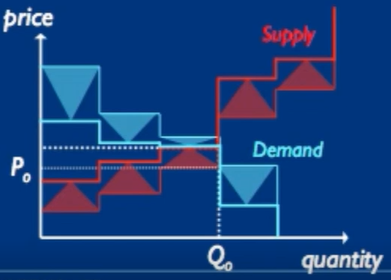
\includegraphics[width=.3\textwidth]{quotedPrices.PNG}
    \caption{The arrows show the displacement from an agents hidden price and their quoted price}
    \label{fig_QuotePriceCurve}
  \end{figure}

  \begin{proposition}{Apparent Supply-and-Demand Curves for a CDA Auction}
    We can plot \textit{Quote Prices} from a CDA Auction to produce \textit{``Apparent Supply-and-Demand Curves''} for the market, but ordering the buy prices in decreasing order and the sell prices in increasing order. In practice these curves are stepped as discrete quantities are offered by each agent.
    \par Any prices to the left of the equilibrium (intersect) are able to exchange in the market or increase their margin, whereas those to the right of the equilibrium will need to decrease their margin in order to make a trade.
  \end{proposition}

  \begin{remark}{No-One Trades their Marginal Price}
    In practice producers do not want to sell at their minimum price (i.e. marginal cost), nor do consumers want to buy at their maximum price (i.e. private value). To avoid paying these prices agents will quote a price some distance away. This produces \textit{``Apparent Supply-and-Demand Curves''} made up of these \textit{quote prices} (See \texttt{Figure 1.\ref{fig_QuotePriceCurve}}).
    \par Some agents will be able to trade at these \textit{quote prices} and those that don't will use them to help inform their next price. The expectation is for the distance between quote and marginal price to decrease over time.
  \end{remark}

  \begin{definition}{Long Selling}
    \textit{Long Selling} is when an agent buys a security with the intention to sell it at some point in the future. You \textit{Long Sell} somethign you expect to \textit{increase} in value.
  \end{definition}

  \begin{definition}{Short Selling}
    \textit{Short Selling} is when an agent $A$ borrows a security from agent $B$, agent $A$ then sells the borrow security to another agent $C$. $A$ will at some point in the future need to buy an equivalent security in order to reimburse $B$. $A$'s hope is that the price of the security will have decrease in this time.
    \par You \textit{Short Sell} something you expect to \textit{decrease} in price. \textit{Short Selling} can be used as insurance/mitigation against market events.
  \end{definition}

  \begin{definition}{Arbitrage}
    \textit{Arbitrage} is the act of simultaneously buying \& selling across markets to make a risk-free profit. This occurs when the price you can buy an asset in one market, is less than the price it can be sold for in another.
    \par \textit{Arbitrage} opportunities don't last for long as the increased demand for the products which make it up will cause the both their prices to contract together.
  \end{definition}

  \begin{table}
    \begin{tabular}{|c|c|p{\dimexpr 0.6\linewidth-2\tabcolsep}|}
      \hline
      \textbf{Acronym}&\textbf{Order Type}&\textbf{Description}\\
      \hline
      MO&\textit{Market Order}&Buy/Sell a defined number of shares at the current market rate.\\\hline
      LIM&\textit{Limit Order}&Buy/Sell a defined number of shares at a specified limit price, or better.\\\hline
      GFD&\textit{Good For Day}&A \textit{Limit Order} which expires at the end of the trading day.\\\hline
      FOK&\textit{Fill Or Kill}&The order only executes if it can be fully filled immediately.\\\hline
      AON&\textit{All Or Nothing}&The order only executes if it can be fully filled, but not necessarily immediately.\\\hline
      IOC&\textit{Immediate Or Cancel}&The order must be executed immediately, but not necessarily in full.\\\hline
      ICE&\textit{Iceberg}&Execute a large order as a sequence of smaller orders.\\\hline
      LOO&\textit{Limit On Open}&A \textit{Limit Order} which is added to the market when it opens.\\\hline
      LOC&\textit{Limit On Close}&A \textit{Limit Order} which is added to the market when it closes.\\\hline
      MOO&\textit{Market On Open}&A \textit{Market Order} which is added to the market when it opens\\\hline
      MOC&\textit{Market On Close}&A \textit{Market Order} which is added to the market when it closes.\\\hline
      OCO&\textit{One-Cancels-Other}&A pair of orders, if one is fulfilled then the other is cancelled.\\\hline
      OSO&\textit{One-Sends-Other}&A pair of orders, once the first is executed the second is sent to the market.\\\hline
    \end{tabular}
    \caption{Selection of common order types available in stock markets.}
    \label{tab_OrderTypes}
  \end{table}

  \begin{proposition}{Order Types}
    There are several different types of orders which can be made in a stock market. Each type requires the agent to specify a price and quantity, but then offer further options to specify: how an order is filled (fully or partially); when the order is cancel; or, further orders to send (See \texttt{Table \ref{tab_OrderTypes}}).
  \end{proposition}

  \begin{definition}{Dark Pool}
    A \textit{Dark Pools} is a marketplace where participants do not want to give away their personal identity. Typically this is because if their identity was known the value of the product would change (e.g. a CEO selling shares in their company).
    \par The identities of participants is only known by the dark pool operator, and there are examples of operators blackmailing/extorting participants.
  \end{definition}

  \begin{remark}{Dark Pools in Practice - Turquoise LSE}
    \textit{Turquoise} is a sub-exchange of the LSE and has two LOBs: \textit{Turquoise Lit}, a standard LOB; and \textit{Turquoise Plato}, a \textit{Dark Pool} where the LOB is not published. %Only sufficiently large orders are routed through \textit{Turquoise Plato} and orders are processed with size priority.
    \par \textit{Turquoise Plato} has two interesting features
    \begin{itemize}
      \item \textit{Uncross} - Orders are allowed to accumulate on the LOB and at random intervals (~5-10 seconds) bids \& offers are matched, in a so-called \textit{Uncross Event}.
      \item \textit{Block Discovery Process} - Agents are allowed to place large, confidential, non-binding orders called \textit{Blocks}, with a specified minimum-size they are willing to accept as a partial fulfilment of their order.
      \par Between \textit{Uncross Events} the owners of matched blocks are asked to confirm their order (An \textit{Order Submission Request}, OSR). The owners are then expected to respond with a firm order (A \textit{Qualifying Block Order}, QBO), which if done means the orders can be completed by the exchange.
      \par Agents can pull out of \textit{Block} orders after receiving an \textit{OSR}, but this will negatively affect their \textit{reputation score} which may lead to them being denied access to the \textit{Block Discovery Process}.
    \end{itemize}
  \end{remark}

\subsection{Market Metrics} \label{sec_MarketMetrics}

\subsection*{Price Description}

  \begin{definition}{Bid-Offer Spread}
    The \textit{Bid-Offer Spread} of a market is the absolute difference in value between the highest bid price and the lowest ask price.
    \[ \text{B-O Spread}:=\big|\min(P_\text{ask})-\max(P_\text{bid})\big| \]
  \end{definition}

  \begin{definition}{Mid-Price}
    The \textit{Mid-Price} of a market is the midpoint between the highest bid price and the lowest ask price (independent of the quantities available at each price).
    \[ \text{Mid-Price}:=\frac12\big(\min(P_\text{ask})+\max(P_\text{bid})\big) \]
    The \textit{Mid-Price} is an estimate of the \textit{Market Equilibrium Price}, but single stray prices can make it stray significantly.
  \end{definition}

  \begin{definition}{Micro-Price}
    The \textit{Micro-Price} of a market is the weighted mean of the highest bid price and the lowest ask price, each weighted by the quantity available at the other order-type (ie bid by ask, and ask by bid).
    \[ \text{Micro-Price}:=\frac{Q(P_\text{max bid})\cdot P_\text{min ask}+Q(P_\text{min ask})\cdot P_\text{max bid}}{Q(P_\text{max bid})+Q(P_\text{min ask})} \]
    where $Q(\cdot)$ is the quantity available at a given price and order-type (bid xor ask).
  \end{definition}

  \begin{definition}{Price Depth}
    \textit{Price Depth} is the number of price levels currently being quoted for a particular product, for a specific order-type (bid xor ask).
  \end{definition}

  \begin{definition}{Volume Depth}
    \textit{Volume Depth} is the total quantity available of a given product, across a specific order-type (bid xor ask).
  \end{definition}

\subsection*{Market Efficiency}

  \begin{definition}{Smith's $\alpha$}
    \textit{Smith's $\alpha$} is a metric of the variation of transaction prices $\{P_t\}_{t\in T}$ around the theoretical equilibrium price $P_0$. This is normalised to be a percentage.
    \[ \alpha:=\frac{100}{P_0}\sqrt{\frac1{|T|}\sum_{t\in T}(P_t-P_0)^2} \]
    Lower values of \textit{Smith's $\alpha$} are better as they indicate a greater concentration of prices
  \end{definition}

  \begin{definition}{Allocative Efficiency}
    \textit{Allocative Efficiency} is a metric of how effective a market is at extracting \textit{Surplus} for its agents $A$. This is normalised to be a percentage.
    \[ 100\times\frac{\sum_{a\in A}S_a}{\text{Theoretical Max. Total Surplus}} \]
    where $S_a$ is the surplus earned by agent $a$.
  \end{definition}

  \begin{definition}{Single Agent Efficiency}
    \textit{Single Agent Efficiency} is a metric for how well an individual agent $a$ performs in a market, compared to other agents. (ie how much surplus $S_a$ they receive compared to other agents). This is normalised to be a percentage.
    \[ 100\times\frac{S_a}{\expect[S_A|P_0]} \]
    where $\expect[S_A|P_0]$ is the expected surplus if all trades occur at price at the theoretical equilibrium $P_0$.
  \end{definition}

  \begin{remark}{Is Intelligence Required for Allocative Efficiency?}
    \textit{Experimental Economics} has demonstrated that very simple \textit{Zero-Intelligence Agents} (ZIC), which quote random prices which do not exceed their assigned limit price, trade in a very human-like manner. Suggesting that most of the intelligence required for a market to be efficient is in the market mechanisms, not the traders.
  \end{remark}

\subsection{Options Markets} \label{sec_OptionsMarkets}

  \begin{definition}{Derivative Contracts}
    A \textit{Derivative Contract} is based on the \textit{Marginal Change} in the value of an asset (the difference in price at two points in time), rather than the absolute value of the asset. \textit{Derivative Contracts} do not require you to own the asset.
    \par Here are two types of \textit{Derivative Contracts}
    \begin{itemize}
      \item \textit{Futures Contract} - Have a \textit{Forward Price} and a \textit{Delivery Date}. The transaction \underline{must} occur on the delivery date, for the forward price (Common in crop yields).
      \par Buyers of a \textit{Future} take a long position (expect the asset to appreciate) while sellers take a \textit{Short} position (expect the asset depreciate).
      \item \textit{Options Contract} - Have a \textit{Strike Price} and a \textit{Delivery Date}. The transaction \underline{may} occur on the delivery date, for the strike price (ie there is no obligation).
      \item There is also \textit{Forwards} and \textit{Swap} contracts.
    \end{itemize}
  \end{definition}

  \begin{remark}{Futures \& Options are Standardised and Exchange Tradable}
    Both \textit{Futures \& Options Contracts} are said to be \textit{Standardised} as the price and delivery date of the contracts are prespecified. This means they can be traded on exchanges.
    \par It is important for these contracts to be \textit{Exchange Tradable} so that investors who do not have the cash to exercise the full value of their contract\footnote{i.e. Buy the amount of the underlying asset they have the right to. In this case your only cost is the commission for buying the contract, and not in actually exercising the contract. You receive (part of) the profit from realising the contract. } can still realise the value of it (by selling to someone who can afford to exercise the option).
  \end{remark}

  \begin{remark}{Betting Exchanges}
    \textit{Betting Exchanges} are similar to \textit{Options Markets} as they allow people with differing views about some future outcome to wager on it. Similarly, the winner makes a profit but the loser loses their whole investment (Whereas, in a stock-market, the loser can recoup some of their investment by selling the asset.).
  \end{remark}

\subsubsection{Options} \label{sec_Options}

  \begin{proposition}{Pricing an Option}
    There are a few factors of an \textit{Options Contract}:
    \begin{itemize}
      \item \textit{Intrinsic Value} - The amount of money exchange if the option is exercised.
      \item \textit{Volatility Premium} - The volatility in the value of the underlying asset.
      \item \textit{Time Value} - How long until the exercise date
    \end{itemize}
  \end{proposition}

  \begin{remark}{Commissions}
    Commissions are paid to set up an \textit{Options Contract}. Commission grows linearly with the number of contracts. You need to make a certain amount of profit on the contract in order to cover all costs.
  \end{remark}

  \begin{remark}{American \& European Style Options Contracts}
    There are two styles of \textit{Options Contracts} which affect how the contract can be exercised.
    \begin{itemize}
      \item \textit{American Style} - The contract can be exercised on \underline{any day} upto the \textit{Delivery Date}.
      \item \textit{European Style} - The contract can be exercised \underline{only} on the \textit{Delivery Date}.
    \end{itemize}
  \end{remark}

  \begin{definition}{Gearing}
    Buy an options contract is much cheaper than buying the underlying asset, this means you can buy more options contracts and thus increase the amount of profit/loss you can make for the same investment. This is known as \textit{Gearing}, and is inherently more risky than buying the underlying asset as if the price does not go in the direction you desire you loss your entire investment.
  \end{definition}

  \begin{figure}[ht!]
    \centering
    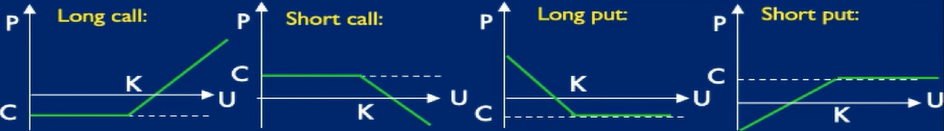
\includegraphics[width=.9\textwidth]{options.PNG}
    \caption{Payoff diagrams for the four basic options contracts.{\tiny $K$ is the \textit{Strike Price}, the green line plots the payoff to the agent $P$ depending on the underlying value of the asset $U$ on the delivery date.}}
    \label{fig_OptionsPayoff}
  \end{figure}

  \begin{proposition}{Types of Options Contract}
    There are two types of \textit{Options Contract}, depending on whether you want the right to buy or to sell.
    \begin{itemize}
      \item \textit{Call Option} - Gives the holder the right to \underline{buy} a set amount of the underlying asset, on some future date, at a specified \textit{Strike Price}. The holder is in the money if the value of the underlying asset is greater than the \textit{Strike Price} on the delivery date.
      \item \textit{Put Option} - Gives the holder the right to \underline{sell} a set amount of the underlying asset, on some future date, at a specified \textit{Strike Price}. The holder is in the money if the value of the underlying asset is less than the \textit{Strike Price} on the delivery date.
    \end{itemize}
    Each of these contracts has two positions an agent can take
    \begin{itemize}
      \item \textit{Long Position} - The holder of the option (ie the agent with the right to buy/sell at the agreed price).
      \item \textit{Short Position} - The writer of the option (ie the agent who \underline{must} buy from/sell to the holder, if the holder wishes to exercise the option).
    \end{itemize}
    This gives four different options contract positions an investor can enter into: Long Call; Short Call; Long Put; or, Short Put. Each of these have different pay offs depending on the change in value of an asset. See \texttt{Figure \ref{fig_OptionsPayoff}}.
  \end{proposition}

  \begin{remark}{Cash Flow Short vs Long Position}
    Agents taking \textit{Long Positions} pay a commission to the agent taking the \textit{Short Position}. This commission is the only way for the \textit{Short Position} agent to make money, whereas the \textit{Long Position} agent makes money depending on the value of the asset on the delivery date.
    \par The commission is the maximum amount the \textit{Long Position} agent can lose, but the maximum amount hte \textit{Short Position} agent can make.
    \par Due to the commission the initial cash-flow is negative for \textit{Long Positions} and positive for \textit{Short Positions} (as seen in \texttt{Figure \ref{fig_OptionsPayoff}}).
  \end{remark}

\subsubsection{Option Strategies} \label{sec_OptionStrategies}

  \begin{definition}{Option Strategies}
    \textit{Option Strategies} are linear combinations of Long Calls; Short Calls; Long Puts and Short Puts. \textit{Option Strategies} are used to limit potential losses/profits, or to allow an agent greater flexibility in the position they are taking.
    \par Below is a table of a selection of \textit{Option Strategies} (For figures see \texttt{\ref{sec_ReferenceOptionStrategies} Options Strategies})

    \begin{adjustwidth}{-1.5cm}{}
      \begin{tabular}{|c|l|l|l|}
        \hline
        \textbf{Name}&\textbf{Description}&\textbf{Constituent Contracts}&\textbf{Fig}\\
        \hline
        Bull Spread&Bounded profit and loss for a forward position.&i) Long call at $K_1$&\ref{fig_BullSpread} \\
        &&ii) Short call at $K_2$&\\\hline

        Bear Spread&Bounded profit and loss for a short position.&i) Short put at $K_1$&\ref{fig_BearSpread}\\
        &&ii) Long call at $K_2$&\\\hline

        Long Butterfly&Profit if underlying value does \underline{not} move,&i) Long call at $K_1$&\ref{fig_LongButterfly}\\
        &bounded loss otherwise.&ii) 2x Short calls at $K_2$&\\
        &&iii) Long call at $K_3$&\\\hline

        Short Butterfly&Bounded profit if underlying value moves,&i) Short call at $K_1$&\ref{fig_ShortButterfly}\\
        &in either direction.&ii) 2x Long calls at $K_2$&\\
        &&iii) Short call at $K_3$&\\\hline

        Long Straddle&Unbounded profit if underlying value changes,&i)Long call at $K_1$&\ref{fig_LongStraddle}\\
        &in either direction&ii) Long put at $K_1$&\\\hline

        Short Straddle&Profit if underlying value does \underline{not} move,&i)Short call at $K_1$&\ref{fig_ShortStraddle}\\
        &unbounded loss otherwise.&ii) Short put at $K_1$&\\\hline

        Long Strangle&Unbounded profit if the underlying value moves&i) Long put at $K_1$&\ref{fig_LongStrangle}\\
        &more than some specified amount, in either direction.&ii) Long call at $K_2$&\\\hline

        Short Strangle&Profit if the underlying value does \underline{not} move&i) Short put at $K_1$&\ref{fig_ShortStrangle}\\
        & more than some specified amount,&ii) Short call at $K_2$&\\
        &otherwise unbounded loss.&&\\\hline

        Ratio Call Spread&Profit if the underlying value does \underline{not} move.&i) Short call at $K_1$&\ref{fig_RatioCallSpread}\\
        &Loss bounded if underlying value decreases but,&ii) 2x Long calls at $K_2$&\\
        &unbounded if value increases.&&\\\hline

        Ratio Put Spread&Profit if the underlying value does \underline{not} move.&i) 2x Short Puts at $K_1$&\ref{fig_RatioPutSpread}\\
        &Loss unbounded if underlying value decreases but,&ii) Long Put at $K_2$&\\
        &bounded if value increases/&&\\\hline

        Ratio Call Backspread&Profit if the underlying value moves:&i) Short call at $K_1$&\ref{fig_RatioCallBackspread}\\
        &Bounded profit if underlying value decreases;,&ii) 2x Long Calls at $K_2$&\\
        &Unbounded profit if underlying value increases.&&\\\hline

        Ratio Put Backspread&Profit if the underlying value moves:&i) Short Put at $K_1$&\ref{fig_RatioPutBackspread}\\
        &Unbounded profit if underlying value decreases;&ii) 2x Long Put at $K_2$&\\
        &Bounded profit if underlying value increases.&&\\\hline
      \end{tabular}
    \end{adjustwidth}
  \end{definition}

  \begin{remark}{Combining Option Contracts}

  \end{remark}

\subsection{Trading Algorithms} \label{sec_TradingAlgorithms}

  \begin{definition}{Automated Trading Algorithms}
    \textit{Automated Trading Algorithms} are algorithms which trade on behalf of an agent in a market. These algorithms are given a limit price and are tasked to maximise their operators surplus. The algorithms have access to the prices offered by other agents in the market, but not their private-value/limit-price.
    \par Here are a selection of \textit{Trading Algorithms}, which represent a timeline progression of these algorithms
    \begin{itemize}
      \item \textit{Zero Intelligence (ZI)} - Offer prices at random, ignoring private-value/limit-price. (Useless).
      \item \textit{ZI-Constrained (ZIC)} - Offer prices at random but never offer prices which would result in a negative surplus for the operator.
      \item \textit{ZI-Plus (ZIP)} - Use machine learning to adapt how far away the prices it offers are from its assigned limit price, given actions in the market.
      \item \textit{Kaplan's Sniper} - Waits until sufficient information is known about the market before offering a price. The aim is for this price to ``snipe'' other prices late into the trading window.
      \item \textit{Gjerstad-Dickhaut (GD)}
      \item \textit{Modified GD (MGD)}
      \item \textit{Extended GD (GDX)}
      \item \textit{Adaptive-Aggressive (AA)}
    \end{itemize}
  \end{definition}

  \begin{definition}{ZIP Traders}
    The \textit{ZI-Plus} algorithm uses machine learning to adapt how far away the prices it offers are from its assigned limit price, given actions in the market.
    \par Let $L$ be the limit price of the agent, $p(t)$ be the price offered be the agent at time $t$ and $q(t)$ be the last quoted price in the market (ie from any agent). $\mu(t)$ is a parameter we seek to learn which models the profit margin the agent tries to make. We define the following learning rules
    \[\begin{array}{rclll}
      \Delta(t)&:=&\beta(T(q(t))-p(t))&\quad&\text{Step towards target}\\
      \Gamma(0)&:=&0&&\text{Initial Momentum}\\
      \Gamma(t+1)&:=&\gamma\Gamma(t)+(1-\gamma)\Delta(t)&&\text{Build momentum towards target}\\
      \mu(t+1)&:=&\frac1L(p(t)+\Gamma(t))-1&&\text{New margin}\\
      p(t)&:=&L(1+\mu(t))&&\text{New price}
    \end{array}\]
    Here $\beta$ is a learning rate parameter, $\gamma$ is a damping parameter and $T(\cdot)$ is a stochastic function of the last quoted market price $q(t)$. ($T(\cdot)$ is the ``target value'' which aims to be slightly better than the last quoted price).
  \end{definition}

  \begin{definition}{Kaplan's Sniper}
    \textit{Kaplan's Sniper} trading algorithm waits until one of the following conditions is met before offering a price (and only offers a price if the achieved margin is above a defined threshold).
    \begin{enumerate}
      \item The \textit{Bid-Offer Spread} is sufficiently small.
      \item Offers are better than the best transaction prices from the previous trading period.
      \item There is a only a short time left in the trading period.
    \end{enumerate}
    This algorithm is based around not giving information away and hopes that the price offered will ``snipe'' all existing offers (and other traders will not have time to react).
  \end{definition}

  \begin{remark}{Kaplan's Sniper \& the Market}
    \textit{Kaplan's Sniper} does not adapt to market activity (ie its threshold do not change) and does not help the market achieve an equilibrium.
    \par \textit{Kaplan's Sniper} relies on other traders being active in order to be effective. A market full of snipers would be very inefficient.
  \end{remark}

  \begin{definition}{GD Traders}
    The \textit{Gjerstad-Dickhaut} (GD) trading algorithm produces an estimate of the probability $f(p)$ of a given price $p$ being accepted and then quotes the price $p_\text{quote}$ which maximises the agent's expected gain.
    \[ p_\text{quote}:=\argmax_{p}p\cdot f(p;H) \]
    \par The belief function for price $p$, given a history of quote prices $H$, is defined as
    \[ f(p;H)=\frac{\text{acc}(p;H)+\text{off}(p;H)}{\text{acc}(p;H)+\text{off}(p;H)+\text{rej}(p;H)} \]
    where $\text{acc}(p;H)$ is the number of bids made below price $p$ which were \underline{accepted} during $H$; $\text{off}(p;H)$ is the number of offers made below price $p$ during $H$; and, $\text{rej}(p;H)$ is the number of bids made above price $p$ which were \underline{rejected} during $H$.
  \end{definition}

  \begin{remark}{GD Belief Function in Practice}
    The belief function $f(p;H)$ used by \textit{GD Traders} is a stepped function, but, in practice, a cubic-spline interpolation is used to smooth the function.
  \end{remark}

  \begin{definition}{MGD Traders}
    The \textit{Modified GD} (MGD) trading algorithm modifies the belief function $f(p;H)$ st it shows zero probability for bids lower than the previous lowest trade price and for offers greater than the previous greatest trade price. This reduces volatility
    \[\begin{array}{rcl}
      f_\text{bids}(p;H)&=&\begin{cases}
      0&\text{if }p<\min(H_\text{acc})\\
      \frac{\text{acc}(p;H)+\text{off}(p;H)}{\text{acc}(p;H)+\text{off}(p;H)+\text{rej}(p;H)}&\text{otherwise}
      \end{cases}\\
      f_\text{offer}(p;H)&=&\begin{cases}
      0&\text{if }p>\max(H_\text{acc})\\
      \frac{\text{acc}(p;H)+\text{off}(p;H)}{\text{acc}(p;H)+\text{off}(p;H)+\text{rej}(p;H)}&\text{otherwise}
      \end{cases}
    \end{array}\]
    where $H_\text{acc}$ is the set of prices where trades were successful made in $H$.
  \end{definition}

  \begin{definition}{GDX Traders}
    The \textit{GDX} trading algorithm is an extension of the \textit{GD} algorithm which introduces \textit{real-time dynamic programming} to formulate bidding strategies in auctions which are characterised by sequential bidding and continuous clearing (e.g. CDA).
    \par The \textit{Dynamic Programming} considers the ``state'' of the agent (their current holdings) and calculates transition probabilities to other states using the market event history $H$ and an algorithm similar to the belief algorithm $f(p;H)$ used in \textit{GD}.
  \end{definition}

  \begin{definition}{Adaptive-Aggressive Traders}
    The \textit{Adaptive-Aggressive} (AA) trading algorithm uses an \textit{Aggressiveness Parameter} which represents an agent's willingness to trade-off profit for actually transacting (more aggressive prices are more likely to be accepted). The underlying \textit{Aggressiveness Function} is updated using \textit{Smith's $\alpha$} (A estimate of market volatility). In a more volatile market, a small change in aggressiveness leader to a greater change in bidding behaviour.

    \par The weighted moving average of previously accepted trades is used to estimate the current market equilibrium price $\hat{P}_0$ and \textit{Smith's $\alpha$}. The estimate $\hat{P}_0$ is used to determine whether the current quoted price $p(t)$ is intra-marginal (ie aggressive) or extra-marginal (ie not aggressive).
  \end{definition}

  \begin{remark}{Algorithms vs Humans}
    % ZIP \& GD are better than humans in terms of average efficiency
  \end{remark}

  \begin{remark}{Comparing Trading Algorithms}
    Performing a full \textit{Analytical Analysis} of the capabilities of each trading algorithm (e.g. using game-theory) is either so difficult that it may as well be impossible or require too many simplifications for the findings to be relevant.
    \par Thus, an \textit{Empirical Analysis} (e.g. simulation experiments) are much more appropriate. There are several simulations which can be inciteful for assessing an algorithms ability to make a market efficient
    \begin{itemize}
      \item \textit{Market Homogeneous} - All agents use the same algorithm. Varying the supply and demand dynamics can be interesting.
      \item \textit{One-in-many} - Where one traders uses algorithm $A$ while all other traders use algorithm $B$. This assesses vulnerabilities in a homogeneous market of $B$ and the ability of $A$ to exploit such a market.
      \item \textit{Balanced-Groups} - An equal proportion of traders use each algorithm (with the same distribution of limit prices for each group for fairness).
    \end{itemize}
  \end{remark}

  \begin{remark}{Market Homogeneity}
    For most applications, including financial markets, \textit{Market Homogeneity} is implausible. There are some scenarios, such as \textit{Market-Based Resource Allocation} (e.g. resources in a network) where it is reasonable to assume that all traders use the same algorithm due to the centralised nature of these scenarios.
  \end{remark}

  \begin{table}[ht!]
    \centering
    \begin{tabular}{|c|c|c|}
      \hline
      &\textit{Market Homogeneous}\\
      \hline
      ZIC&Slow but did converge\\
      Sniper&No convergence\\
      ZIP&Converged quickly\\
      MGD&Converged quickly\\
      \hline
    \end{tabular}
    \caption{Description of how each algorithm performed in a homogeneous market.}
    \label{tab_HomogeneousMarket}
  \end{table}

  \begin{table}[ht!]
    \centering
    \begin{tabular}{|c|c|c|c|c|c|}
      \hline
      &Many ZIC&Many Sniper&Many ZIP& Many GD&Many MGD\\
      \hline
      One ZIC&-&-.238&-.124&-.005&-.105\\
      One Sniper&.011&-&.011&.068&.018\\
      One ZIP&.091&.117&-&.028&-.022\\
      One GD&.130&-.039&-.290&-&-\\
      One MGD&.158&.235&-.162&-&-\\
      \hline
    \end{tabular}
    \caption{The average improvement of introducing a single agent with a different algorithm to a homogenous market}
    \label{tab_OneInMany}
  \end{table}

  \begin{table}[ht!]
    \tiny\centering
    \begin{tabular}{|c|c|c|c|c|c|}
      \hline
      (Wins)&ZIC&ZIP&Sniper&GD&MGD\\
      \hline
      ZIC&-&0-100&100-0&1-99&1-99\\
      ZIP&100-0&-&99-1&63-36&29-71\\
      Sniper&0-100&1-99&-&7-93&2-98\\
      GD&99-1&36-63&93-7&-&-\\
      MGD&99-1&71-29&98-2&-&-\\
      \hline
    \end{tabular}
    \begin{tabular}{|c|c|c|c|c|c|}
      \hline
      (Efficiency)&ZIC&ZIP&Sniper&GD&MGD\\
      \hline
      ZIC&-&.955&.964&.978&.960\\
      ZIP&.955&-&.982&.996&.997\\
      Sniper&.964&.982&-&.978&.993\\
      GD&.978&.996&.978&-&-\\
      MGD&.960&.997&.993&-&-\\
      \hline
    \end{tabular}
    \caption{Results of a balanced-group simulation}
    \label{tab_BalanceGroup}
  \end{table}

  \begin{proposition}{Trading Algorithm Performance}
    \texttt{Tables \ref{tab_HomogeneousMarket}, \ref{tab_OneInMany}, \ref{tab_BalanceGroup}} provide summaries of how the trading algorithms performed in the tests described in \texttt{Remark 2.9}.
    \par \texttt{Table \ref{tab_OneInMany}} shows that introducing a \textit{ZIC} trader always reduces market efficiency; Introducing a \textit{Sniper} always improves market efficiency; Introducing a \textit{ZIP} trader improves market efficiency unless the rest of the market use \textit{MGD}; And, similarly, introducing a \textit{MGD} trader improves market efficiency unless the rest of the market use \textit{ZIP.}
    \par \texttt{Table \ref{tab_BalanceGroup}} shows that \textit{MGD} is the superior algorithm in a \textit{Balanced Group} simulation. It has been shown that \textit{AA} traders outperforms GDX \& ZIP in \textit{Balanced Group} simulations, but is not dominant (ie there are some ratio of groups where \textit{AA} doesn't win. See \texttt{Figure \ref{fig_DominantStrategy}}).
  \end{proposition}

  \begin{figure}[ht!]
    \centering
    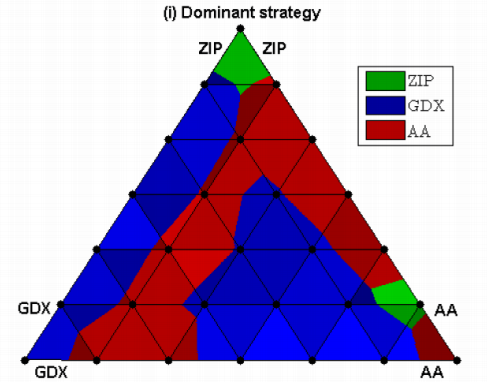
\includegraphics[width=.3\textwidth]{DominantStrategy.PNG}
    \caption{Which trading algorithm wins for different mixtures of the population. None is dominant!}
    \label{fig_DominantStrategy}
  \end{figure}

\subsection{Prediction Markets} \label{sec_PredictionMarkets}

  \begin{definition}{Prediction Markets}
    \textit{Prediction Markets} are an exchange-traded market which attempt to draw on the \textit{Wisdom-of-crowds} to determine the outcome of a future events. Agents in the market are able to trade \textit{``coupons''} which will payout if a particular outcome occurs (e.g. a particular party wins an election). As this is a free market and agents are only motiviated by finances (not political preference), the outcomes the crowd deems more likely should eventually be priced higher.
    \par The payout of these \textit{``coupons''}
    \begin{itemize}
      \item \textit{Winner-Takes-All} - A fixed value is payed if a particular event occurs.
      \item \textit{Vote-Share} - The amount payed out depends on a quantitative outcome (e.g. Number of seats won in an election).
    \end{itemize}
    The total price of all the \textit{``coupons''} should equal the total payout.
  \end{definition}

\section{Economics of the Internet}\label{sec_EconomicsOfTheInternet}

  \begin{definition}{Network Externality}
    A \textit{Network Externality} are non-monetary effects which occur to a consumer due to other consumers using compatible products. Products with positive network externalities are known as \textit{Network Goods}.
    \par Phones have \textit{Network Externalities}. The more people that own a phone the more people you can call with yours. Conversely, if no-one else owns a phone then yours is effectively uselss.
  \end{definition}

  \begin{remark}{Network Externalities - Positive Feedback Loop}
    \textit{Positive Network Externalities} can produce a \textit{Positive Feedback Loop} where consumers choose to buy produces with are compatible with their friends, rather than necessarily the best product (AKA \textit{Brand Value}). This increases the size of the network and thus the magnitude of the \textit{Positive Network Externalities}.
  \end{remark}

  \begin{figure}[ht!]
    \centering
    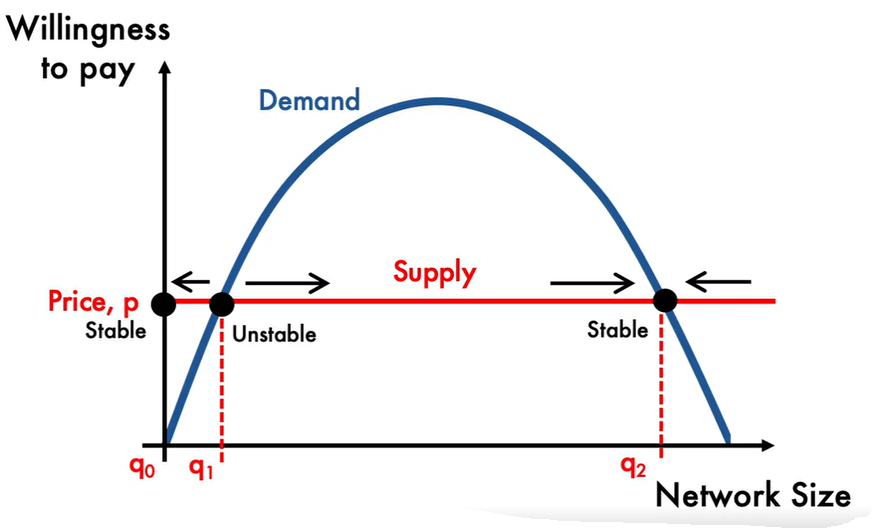
\includegraphics[width=.5\textwidth]{networkDemandCurve.PNG}
    \caption{Network Effect Demand Curve.}
    \label{fig_NetworkEffectDemandCurve}
  \end{figure}

  \begin{definition}{Network Effect Demand Curve}
    A \textit{Network Effect Demand Curve} shows the price consumers are willing to pay for a product given the size of the network using that product (See \texttt{Figure \ref{fig_NetworkEffectDemandCurve}}). A \textit{Network Effect Demand Curve} has an upside-down $U$ shape.
    \par The gradient of the \textit{Network Effect Demand Curve} is initially positive as the \textit{Marginal Value} of each extra user is higher, but this diminishes as the network grows.
  \end{definition}

  \begin{proposition}{Equilibria Points of a Network Effect Demand Curve}
    For any price $P$, there are three network sizes which produce equilibria $q_0,q_1,q_2$ on the \textit{Network Effect Demand Curve} (See \texttt{Figure} \ref{fig_NetworkEffectDemandCurve} ). $q_0$ is a network of size $0$ and thus is naturally stable.
    \par $q_1$ is an unstable-equilibria, known as the \textit{Critical Mass}. If the network is larger than $q_1$ then it will grow to size $q_2$, but if it is smaller than $q_1$ it will shrink to $q_0$ (ie non-existent).
  \end{proposition}

  \begin{definition}{Disruptive vs Sustaining Innovation}
    There are two types of innovation:
    \begin{itemize}
      \item \textit{Sustaining Innovations} - Incremental improvements of traditional performance metrics for existing products.
      \item \textit{Disruptive Innovations} - Vast improvement of \textit{non}-traditional performance metrics which generate new markets \& products (Typically underperform on traditional performance metrics).
    \end{itemize}
  \end{definition}

  \begin{definition}{Combinatorial Innovation}
    \textit{Combinatorial Innovation} occurs when multiple innovations can be combined \& recombined to create new innovations. (The Internet is a combinatorial innovation due to its standardised \& open-source nature).
  \end{definition}

  \begin{figure}[ht!]
    \centering
    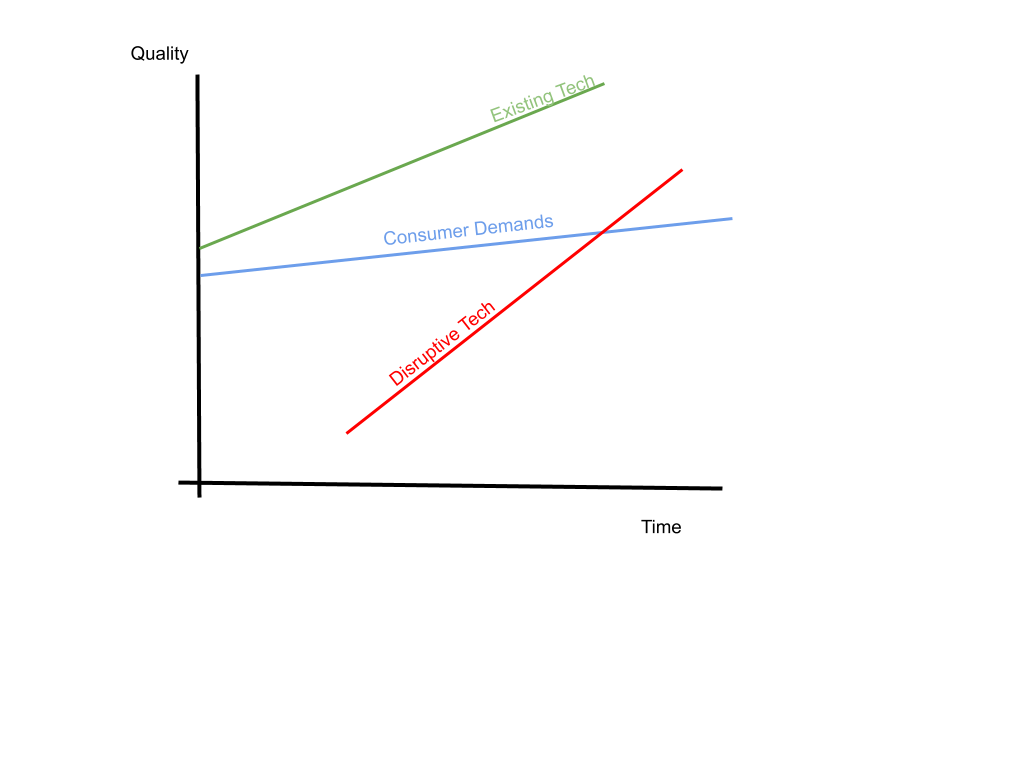
\includegraphics[width=.5\textwidth]{disruptiveTechnology.png}
    \caption{Timeline of how a disruptive technology can establish itself in a market.}
    \label{fig_DisruptiveTechnology}
  \end{figure}

  \begin{remark}{Disruptive Technology - Established Producers}
    Establish companies are typically slow to invest in \textit{Disruptive Technologies} as these new technologies do not meet the needs of the company's clients.
    \par Often, by the time the disruptive technology does reach the requirements of these clients, there is already an establish company in the new market and the original company will struggle to compete. The product of the original company may still be of greater quality than the new technology, but it severely underperforms in the non-traditional performance metrics customers now care about (See \texttt{Figure \ref{fig_DisruptiveTechnology}}).
  \end{remark}

  \begin{remark}{Timeline of Disruptive Technology}
    Here is the typical timeline of a successful \textit{Disruptive Techonology} (As illustrated in \texttt{Figure \ref{fig_DisruptiveTechnology}}).
    \begin{enumerate}
      \item \textit{Disruptive Technology} is invented (Often by an established company).
      \item The \textit{Disruptive Technology} does not meet the needs of the establish company's clients, and thus the company does not focus on the new technology.
      \item New companies form to pursue the \textit{Disruptive Technology} (Often by ex-employees of the established company).
      \item The \textit{Disruptive Technology} sufficiently improves along traditional performance metrics and becomes main-stream/commercially successful.
      \item The establish companies tries to enter the new market but is too late.
    \end{enumerate}
  \end{remark}

  \begin{definition}{Switching Costs}
    \textit{Switching Costs} are costs a customer incurs when switching services, both monetary and non-monetary costs. When \textit{Switching Costs} are too high a customer becomes \textit{Locked-In} as they will choose to stay with an inferior service than incur the switching costs of moving to a better service.
    \par Potential \textit{Switching Costs} include:
    \begin{itemize}
      \item \textit{Setup Costs}.
      \item \textit{Training Costs} - Having to learn a new service.
      \item \textit{Network Effects} - Losing positive network externalities of the existing service.
      \item \textit{Initial Loss in Quality} - The new service will not know you as well as the existing service so may offer inferior services initially (e.g. Show recommendations on Netflix).
    \end{itemize}
  \end{definition}

\subsection{Digital Goods} \label{sec_DigitalGoods}

  \begin{proposition}{Digital vs Physical Goods}
    There are several common economic differences between digital and physical goods
    \begin{itemize}
      \item \textit{Costs}: Digital goods are expensive to produce, but cheap to reproduce. (i.e. High fixed costs, low variable costs).
      \item \textit{Capacity Constraints}: There is no limit to the number of times a digital good be reproduced.
      \item \textit{Sunk Costs}: Investment into digital goods are sunk costs. (i.e. You can recoup costs by selling unneeded shop-buildings, but you cannot recoup the cost of software developer time).
      \item \textit{Ascertaining Value}: Digital goods are more likely to be \textit{Experience Goods}, meaning customers cannot know whether they will like the good before purchasing it. (ie customers cannot assign a value).
      \item \textit{Search Costs}: It is much easier for a customer to search for/compare competing digital products online, than competing physical goods offline.
      \item \textit{Network Externalities}: Digital goods are more likely to have strong positive network externalities.
      \item \textit{Switching Costs}: Digital goods are more likely to have greater switching costs, and try to lock-in customers.
    \end{itemize}
  \end{proposition}

  \begin{figure}[ht!]
    \centering
    \begin{subfigure}[b]{.45\textwidth}
         \centering
         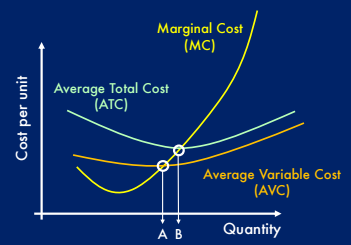
\includegraphics[width=\textwidth]{physicalCostCurve.PNG}
         \caption{Physical Good}
    \end{subfigure}
    \begin{subfigure}[b]{.45\textwidth}
         \centering
         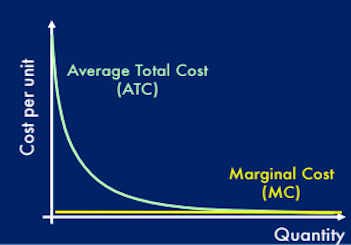
\includegraphics[width=\textwidth]{digitalCostCurve.PNG}
         \caption{Digital Good}
    \end{subfigure}
    \caption{Typical cost curve for physical and digital goods.}
    \label{fig_DigitalCostCurve}
  \end{figure}

  \begin{proposition}{Cost Curve for Digital Goods}
    Digital goods typically have high fixed costs and low variable costs, meaning the \textit{Marginal Cost} of digital goods is effectively zero and average costs tend to zero. The \textit{Cost Curve} for digital and physical goods are very different (See \texttt{Figure \ref{fig_DigitalCostCurve}}).
  \end{proposition}

  \begin{remark}{Minimum Price of Digital Goods}
    As \textit{Digital Goods} have effectively zero \textit{Marginal Cost} producers can justify selling their product for nothing.
    \par They will need to recoup the initial fixed costs at some point in the future. Many businesses give away their product for free until they reach critical mass, at which point they attempt to monetise it.
  \end{remark}

  \begin{remark}{Competition between Producers of Digital Goods}
    Due to very low marginal costs, when there is competition in a market producers of similar digital goods quickly drop their price to zero. This makes it hard for new companies to enter, due to high fixed costs.
    \par Companies will then compete on the quality of their product and try to build positive network externalities, with lock-in.
  \end{remark}

  \begin{definition}{Freemium Business Model}
    The \textit{Freemium Business Model} offers a free version of a digital good and then encourages customers to upgrade to the premium version.
  \end{definition}

  \begin{definition}{File Formats}
    \textit{File Formats} are a standardised ways for encoding digital information. There are often multiple formats for the same type of object (e.g. JPEG v SVG v PNG).
  \end{definition}

  \begin{remark}{Proprietary Formats}
    Some companies choose to encoding their digital information with \textit{Proprietary Formats} (ie formats only their software knows how to read). This increases the switching costs for customers, but reduces the shareability of the information. The reduced shareability is good for some information (e.g. copyrighted-music) but not for others (e.g. word documents).
    \par There are examples (e.g. MS Word's .DOC) of \textit{Proprietary Formats} being reverse engineered by other companies/groups in order to piggy back the network externalities of these products.
  \end{remark}

  \begin{remark}{Industry-Wide Standards}
    Sometimes \textit{Industry-Wide Standards} are agreed, allowing customers to share files between providers. This increases the network effect, likely attracting new customers.
    \par The trade-off for producers is between having a large part of a small pie; or a small part of a large pie.
  \end{remark}

  \begin{proposition}{How Industry-Wide Standards Develop}
    There are three common ways for \textit{Industry-Wide Standards} to develop
    \begin{enumerate}
      \item A single, major, producer sets a standard by opening up their proprietary format(e.g Adobe with PDF).
      \item A \textit{``war''} occurs between multiple producer wishing to set the standard (Generally to the deteriment of all).
      \item Several producers negotiate a standard. There is always a risk that during this process one party will pull out and use their own proprietary format.
    \end{enumerate}
  \end{proposition}

\subsection{Online vs Offline Businesses} \label{sec_OnlineVsOfflineBusinesses}

  \begin{remark}{Laws of Economics are Invariant}
    The \textit{Laws of Economics} (e.g supply-and-demand) are fundamentally the same for online \& offline businesses. It is the characteristics of online business activities which result in different markets.
  \end{remark}

  \begin{figure}[ht!]
    \centering
    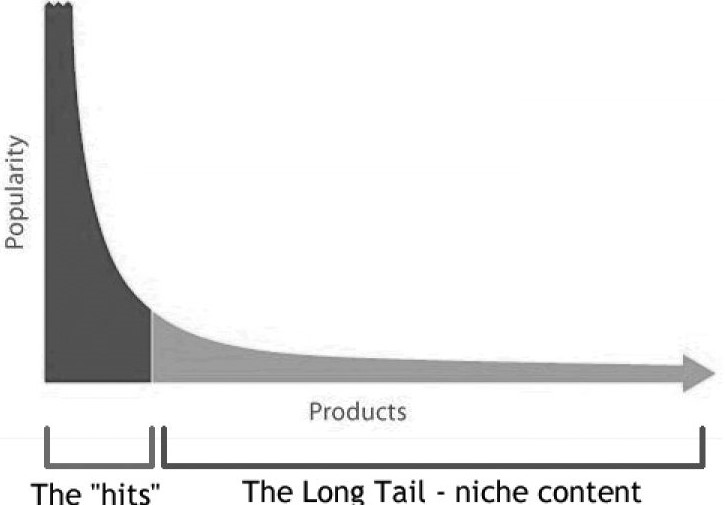
\includegraphics[width=.5\textwidth]{LongTail.jpg}
    \caption{Illustration of how popularity dictates which products are sold.}
    \label{fig_LongTail}
  \end{figure}

  \begin{proposition}{The Long Tail}
    The variety of products an offline business can sell is limited by the shelf space they have. This means that only the best selling products are stocked and sold by the business.
    \par However, online business either have much more space for physical goods (due to using warehouses) or unlimited space if selling digital goods. This means online business can stock a greater variety of products. Moreover, online businesses selling digital goods should offer any product which makes at least one sale as it costs them (almost) nothing to do so (See \texttt{Figure \ref{fig_LongTail}}).
  \end{proposition}

  \begin{proposition}{Utilising the Long Tail}
    There are a few steps an online business can take to utilise the idea of the long tail
    \begin{enumerate}
      \item Make it easy for customers to find new products (ie good recommender systems).
      \item Offer everything, someone will by it.
      \item Reduce prices, as economies-of-scale reduce costs.
    \end{enumerate}
  \end{proposition}

\subsection{Online Price Discrimination Strategies} \label{sec_OnlinePriceDiscriminationStrategies}

  \begin{remark}{Personalised Pricing}
    \textit{Personalised Pricing} is, in-theory, much easier online as producers have more information about their customers. However, it is not believed that any major companies use personalised pricing due to potential public backlash. Rather, they choose to use this information to promote items/sales they believe a customer is more likely to be interested in.
    \par European data protection laws require producers to specify, to their customers, how any data collected is used. This means a company would have to state they use the data for personalised pricing (likely leading to backlash and people trying to game the system).
  \end{remark}

  \begin{remark}{Digital Product Versioning}
    As digital goods have near-zero reproduction costs and software can easily be customised (by blocking access to certain features), \textit{Product Versioning} is common with digital goods.
    \par \textit{Bundling} digital goods together is easy to setup and at very low cost to the producer.
  \end{remark}

  \begin{proposition}{Unbundling}
    Due to it being easy for a customer to purchase digital goods, customers are willing to make lots of small purchases which they may not for physical goods (i.e. you wouldn't and buy penny sweets every day). This can lead to the practice of \textit{Unbundling} where producers sell the components, of what is typically larger product, individually (e.g. articles of a magazine).
  \end{proposition}

\subsection{Economics of Computer Games} \label{sec_EconomicsOfComputerGames}

  \begin{remark}{In Game vs IRL Currencies}
    \textit{In-Game Currencies} are in-essence very similar to IRL currencies, as they are stimulated by players collecting raw materials, producing goods and then trading (Especially in multi-player games).
    \par This means they share similar problems around stability (ie balancing money entering and leaving the system). If this balance is not good then \textit{MUDFlation} occurs (ie inflation). It is important for in-game currencies to be stable otherwise the game's longevity will be shortened.
  \end{remark}

  \begin{remark}{Meta-Currencies}
    In cases where in-game currencies have proven unstable, there are examples of player bases developing \textit{Meta-Currencies} where they decide an alternative unit of trade (e.g. cigarettes/fish in prisons).
  \end{remark}

  \begin{remark}{IRL Value}
    For many popular games there are IRL markets where players sell their in-game assets for Fiat-currencies (This is essentially an FX market).
    % Gold Farming
    \par \textit{Gold Farming} is a practice of players grinding tasks in a game in order to acquire assets they intend to sell in IRL markets. This can prove a profitable endeavour, especially in countries with lower wages. \textit{Gold Farming} typically breaks the EULA of a game but it is hard for game makers to counter.
  \end{remark}

  \begin{remark}{Game Development - Budgets}
    The budget and size of teams involved in creating AAA titles has grown exponentially (Tracking the powerfulness of computers). However, the \textit{average} game budget has decreased as it is easier for individuals to create passion-project games (due to better tools being available).
    \par Interestingly, the mid-size studio (with budges in low millions) have almost disappeared due to them either being absorbed by larger firms or splintering into smaller firms.
  \end{remark}

  \begin{remark}{Game Development - Employee Specialisation}
    As the desired quality of games has increased, employees have become increasing specialised. This means individual tasks now take longer and more people are required to create a high quality game. This increases the production costs.
  \end{remark}

\subsection{Online Auctions} \label{sec_OnlineAuctions}

  \begin{remark}{Online Auctions}
    Due to well-defined rules of auctions and the fact there is no need to have a physical auctioneer, it is easy to write algorithms to perform auctions digitally. Moreover, the internet enables auctions to be run quickly and cheaply with the only limit being server capacity and bandwidth.
    \par It is possible for bidders to automate their bidding process too. This has lead to more complex auctions being introduced.
  \end{remark}

  \begin{remark}{Intermediaries}
    Although the internet makes it viable for small businesses to hold their own auctions, most choose to use an intermediary marketplace (e.g. Amazon \& eBay) due to the greater exposure these intermediaries offer.
    \par These marketplaces also make payments easier and improve trustworthiness of both buyers and sellers.
  \end{remark}

  \begin{definition}{Snipping}
    \textit{Snipping} is the practice of placing bids close to the expiry time of the auction, in the hope that other buyers do not have enough time to outbid you. This means that information about a bidder's \textit{Private Value} is kept secret for as long as possible.
  \end{definition}

  \begin{remark}{Estimating Demand Curves for Online Auctions}
    In online auctions it is easier to track attempted bids\footnote{Some bids may not be accepted due to the price being too high when that bidder enters the market.} you can plot an estimate for the demand curve. This estimate can be used to derive optimal sale strategies and for estimating revenue.
  \end{remark}

  \begin{remark}{eBay}
    \textit{eBay} is an online auctioneer which specialises in consumer-to-consumer and producer-to-consumer auctions (and some business-to-business auctions). \textit{eBay} uses an \textit{Open-Ascending Auction with a Deadline}, this similar to an \textit{English Auction} but has a predefined expiry date.
    \par Reviews of sellers act to \textit{Lock-In} sellers and thus attract buyers, this is in part how \textit{eBay} has an effective monopoly.
  \end{remark}

  \begin{remark}{Snipping on eBay}
    \textit{Snipping} is/was a common practice on \textit{eBay} with specialist software being written to help enable it. To combat this \textit{eBay} introduced a system of \textit{``proxy bidding''} where bidders state the maximum they are willing to bid and the system places the minimum bid required for them to be winning the auction at any point in time (provided this is below the specified maximum). If all bidders use this system then an \textit{eBay} auction becomes an \textit{SPSB Auction} with a time limit.
  \end{remark}

  \begin{remark}{Google Ad Auctions}
    \textit{Google} uses auctions for its \textit{Ad-Space} (multiple auctions per user-search results page). In order to maintain a good user experience, \textit{Google} considers both \textit{bid price} and \textit{advert quality} (assessed by historic click-through rate, relevancy and landing page quality) when choosing the winner of an auction.
    \par Originally \textit{Google} used \textit{FPSB Auctions} but this lead to server overload as bidders checked ther results of auctions (to see if they could lower their pricing). Switching to \textit{SPSB Auctions} solved this issue due to \textit{SPSB Auctions} being incentive compatible.
  \end{remark}

\subsection{The Crowd Economy} \label{sec_TheCrowdEconomy}

  \begin{definition}{Crowd Economy}
    The \textit{Crowd Economy} is the group of platforms which rely on active online=participation from large crowds of people, in order to provide their services (e.g. \textit{Wikipedia} \& \textit{AirBnB}).
  \end{definition}

  \begin{definition}{Crowdsourcing}
    \textit{Crowdsourcing} is the practice of using crowds to complete some task (e.g. image labelling, writing articles). \textit{Crowdsourcing} is often used for tasks which are difficult for a computer to do.
  \end{definition}

  \begin{proposition}{Finding Participants for Crowdsourcing}
    Here are some practices which business can use to encourage participation
    \begin{itemize}
      \item \textit{Pay Them} - Typically only a few pence, as on \textit{Mechancial Turk}.
      \item \textit{Trick Them} - Require them to complete the task to complete something they actually want to (e.g. \textit{Amazon's Mechanical Turk}).
      \item \textit{Motivate Them} - Make the task fun or meaningful (e.g. for medical research).
    \end{itemize}
  \end{proposition}

  \begin{definition}{Crowdfunding}
    \textit{Crowdfunding} is the practice of raising funds for a project (e.g. producing a project) from crowds of people. This can take several forms
    \begin{itemize}
      \item \textit{Donation Based} - Funders give money for no reward, except for good feels.
      \item \textit{Reward Based} - Give funders rewards based on how much they pledge.
      \item \textit{Equity Based} - Funders become share holders.
      \item \textit{Debt Based} - Accept funding from many funders with the agreement to repay with interest (effectively a cheap loan), this is AKA \textit{Peer-to-Peer Funding}.
    \end{itemize}
  \end{definition}

  \begin{remark}{Crowdfunding Regulation}
    In the UK \textit{Equity Based} and \textit{Debt Based Crowdfunding} are regulated by the FCA, in the same way traditional services are.
  \end{remark}

\section{Financial Technology} \label{sec_FinancialTechnology}

  \begin{remark}{The Underbanked}
    \textit{The Underbank} are the $\sim70\%$ of the world, typically outside the western world, do not have access to basic banking facilities. These people are prime customers for \textit{FinTechs}, as these customers desire easy-access and simplicity, over quality products.
    \par More people have access to mobile phones than banking services, so mobile based banking services are particularly attractive. This is why \textit{FinTechs} often focus on mobile-centric services.
  \end{remark}

\subsection{FinTech Firms} \label{sec_FinTechFirms}

  \begin{proposition}{Key Players}
    There are three key types of company which are involved in \textit{Financial Technology}
    \begin{itemize}
      \item \textit{Traditional Financial Services} - Focus on \textit{Incremental Innovation} to improve their traditional business functions and productivity (through \textit{Digitisation}).
      \item \textit{Start Ups} (FinTechs) - Focus on \textit{Disruptive Innovation} in order to create new financial services markets for them to enter.
      \item \textit{Big Tech} (TechFins) - Seek to leverage their existing technological dominance to offer financial services to existing customers. They are able to do this due to their positive network externalities and likely high \textit{Lock-In}.
    \end{itemize}
  \end{proposition}

  \begin{remark}{Regulators vs FinTechs}
    The goal of regulators is to: Protect participants; Improve market competitiveness; And, build trust.
    \par New financial technologies may require new regulation. Some national regulators are more welcoming to new technologies, taking a \textit{``Watch and See''} approach where they allow new technologies to enter the market and then work with the business to implement regulations (Known as \textit{Sandboxing}).
  \end{remark}

  \begin{remark}{China}
    \textit{China} uses a \textit{development-led} approach to new technologies, allowing new technologies to develop first and adding regulation later (once it is clear it is needed).
  \end{remark}

  \begin{remark}{India}
    \textit{India} uses a \textit{development-lagged} approach to new technologies, heavily restricting the ability of new technologies to enter the market before they are well understood.
  \end{remark}

  \begin{definition}{LASIC Principles}
    The \textit{LASIC Principles} are a set of principles, suggested by \textit{Less \& Teo}, a \textit{FinTech} should follow in order to succeed:
    \begin{itemize}
      \item \textit{Low Margin} - Selling services with a \textit{Low Profit Margin} allows the business to service, whilst attracting as many customers as possible.
      \item \textit{Asset Light} - Fewer assets mean lower \textit{Fixed Costs}. Piggy-backing on existing infrastructure (e.g. Mobile Phones) will help.
      \item \textit{Scalable} - Having a business model and technologies which are able to scale, without affecting efficiency or cost, helps build \textit{Positive Network Effects}.
      \item \textit{Innovative} - Innovative technologies encourage customers to adopt your services.
      \item \textit{Compliance Easy} - Not being restricted by regulators helps a business be scalable.
    \end{itemize}
  \end{definition}

  \begin{table}[ht!]
    \begin{tabular}{|p{\dimexpr 0.2\linewidth-2\tabcolsep}|p{\dimexpr 0.45\linewidth-2\tabcolsep}|p{\dimexpr 0.45\linewidth-2\tabcolsep}|}
      \hline
      &\textbf{High Banking Prevalence}&\textbf{Low Banking Prevalence}\\\hline

      &\underline{\textit{Partnering} (e.g. Western Europe)}&\underline{\textit{Tech Dominance} (e.g. China)}\\
      \textbf{High Venture Capital Investment}&Competition is likely to come from outside traditional banking. It is Possible for a \textit{FinTech} to thrive but, it is easier to do so by partnering with an establish bank.&Ideal for \textit{FinTechs} as there is little established competition.\\
      \hline

      &\underline{\textit{Bank Dominant} (e.g. Eastern Europe)}&\underline{\textit{Race-to-Finish} (e.g. Sub-Saharan Africa)}\\
      \textbf{Low Venture Capital Investment}&Most competition occurs between established business, and not form new \textit{FinTechs}.&Telecom companies often the most significant tech-firms in these countries. Meaning mobile phones are the key technology to gaining a foothold in these markets.\\
      \hline
    \end{tabular}
    \caption{Four classes of national banking maturity.}
    \label{tab_BankingMaturity}
  \end{table}

  \begin{proposition}{National Banking Maturity}
    The viability of a new financial technology varies by country, depending on the maturity of its banking infrastructure. There are four main categories countries can fall into (See \texttt{Table \ref{tab_BankingMaturity}}).
  \end{proposition}

\subsection{Blockchain} \label{sec_Blockchain}

  \begin{definition}{Blockchain}
    A \textit{Blockchain} is a list of records \textit{(``blocks'')} where each record contains a hash of the previous record, linking records together in a chain.
  \end{definition}

  \begin{remark}{Storing a Blockchain}
    A \textit{Blockchain} can be stored in a single location, but it is more common for multiple parties to each store different parts of the blockchain (with multiple copies of each part). These parts can be compared to verify the integrity of the \textit{Blockchain}, and as they are distributed it is harded for the \textit{Blockchain} to be changed retrospectively
  \end{remark}

  \begin{remark}{Changing a Blockchain}
    Blockchains are designed to be resistant to modification. Modifying a block will change it's hash and thus all latter blocks would need to be changed as well. This is effectively impossible if there are multiple copies of the blockchain (or parts of it) stored by different parties, as all copies need to be updated and it is unlikely all parties will agree to this.
  \end{remark}

  \begin{proposition}{Forks in a Blockchain}
    A \textit{Fork} occurs in a \textit{Blockchain} if there are two versions currently being circulated. There are defined procedures for what to do in this scenario. In general a longer chain is deemed to be correct.
    \par Suppose block $Z$ is the globally agreed end of the chain and suppose two blocks $A$,$B$ are successfully added onto the blockchain at the same time, by different miners. This means two chains (1) \& (2) are being propagated around the network.
    \[\begin{array}{rl}
      (1)&\dots \to Z\to A\\
      (2)&\dots \to Z\to B
    \end{array}\]
    Suppose a node which currently believes chain (1) to be correct, successfully mins block $C$ onto the chain (3) and propagates it out.
    \[\begin{array}{rl}
      (3)&\dots \to Z\to A\to C
    \end{array}\]
  \end{proposition}
  This will cause a fork for any nodes which currently believe chain (2) to be correct. For these nodes, then will drop their current chain (2) and accept (3) to be the correct chain as it is longer. Eventually, chain (3) will be the globally accepted truth.

  \begin{definition}{Bitcoin}
    \textit{Bitcoin} is a decentralised-cryptocurrency which uses a \textit{Distributed Blockchain} to record transactions.
  \end{definition}

  \begin{remark}{R3}
    \textit{R3} is a consortium of banks which are developing a \textit{Blockchain} technology for recording inter-bank transactions. This has been criticised as \textit{Blockchain} technology is generally much slower and more expensive thatn existing technology.
  \end{remark}

\subsubsection{Road to Bitcoin} \label{sec_RoadToBitcoin}

  \begin{remark}{Early Internet Payments}
    In the early life of the Internet, secure HTTP protocols did not exist. This meant good encryption could not be used, making sending payment details very risky.
  \end{remark}

  \begin{remark}{Road to Bitcoin}
    Here are a few technologies which were part of the learning process which lead to Bitcoin.
    \begin{enumerate}
      \item \textit{Credit-Based Payment Architectures} - An intermediary facilitates payment between the seller and the buyer.
      \item \textit{Cash-Based Payment Systems} - Customers buy \textit{``tokens''} with fiat currencies. These \textit{``tokens''} are then exchanged with sellers, who can the \textit{``tokens''} for fiat currency.
      \item \textit{HashCash} - Users had to complete a cryptographic puzzle in order to send an email. This was to discourage spam emails.
      \item \textit{Ledgers for Timestamping} - A trusted server stories copies of documents along with a timestamp for when the document was received, in order to keep a trusted record.
    \end{enumerate}
  \end{remark}

  \begin{definition}{Credit-Based Payment Architectures}
    \textit{Credit-Based Payment Architectures} are based around an intermediary who facilitates a payment between the seller and the buyer. Typically the intermediary securely stores the payment details of both parties, thus not requiring the parties to share their payment details with each other. When a payment request from one/both parties is received, the intermediary debits the buyer and subsequently credits the seller (Typically after some dispute window).
    \par Here are two popular early implementations \textit{Credit-Based Payment Architectures}
    \begin{itemize}
      \item \textit{FirstVirtual} - A predecessor to \textit{PayPal}. Both buyers and sellers had to be registered with \textit{FirstVirtual}.
      \par To reduce fraud \textit{FirstVirtual} allowed buyers a 90 day dispute window and would not credit sellers until after this window, for this reason \textit{FirstVirtual} was not popular with sellers.

      \item \textit{SET Architecture Standard} - A system developed by \textit{Visa} \& \textit{MasterCard}. Buyers did not have to enrol with the system, rather they install an application on their device which would store their details and when a purchase was made the app would encrypt these details and send to \textit{Visa} or \textit{MasterCard}.
      \par Buyers were required to certify all transactions which was a complicated and time-consuming process, making \textit{SET} unpopular with buyers.
    \end{itemize}
  \end{definition}

  \begin{definition}{Cash-Based Payment System}
    \textit{Cash-Based Payment Systems} allow users to exchange fiat-currencies for digital \textit{``tokens''} and visa-versa. Secure mechanisms are then provided for exchanging the \textit{``tokens''}, and even if these systems are compromised user payment details would not be at risk.
    \par The value of \textit{``tokens''} are typically pegged to a fiat-currency (ie they are not a free floating currency. See \texttt{Remark 4.9}).
    \begin{itemize}
      \item \textit{DigiCash} was a \textit{Cash-Based Payments System} which used \textit{eCash} coins. Owners chose a unique private ID for each of their tokens, this could be as complicated as they liked, and stating this ID was proof of ownership. A centralised databased ensured no double spending.
      \par \textit{DigiCash} failed as sellers were not anonymous (while buyers were), and it did not allow buyer-to-buyer transactions.
    \end{itemize}
  \end{definition}

  \begin{remark}{Free-Floating Currency}
    A currency is \textit{Free-FLoating} if its value is based on its supply-and-demand relative to other currencies, rather than being explicitly being defined in terms of another currency (like most in-game currencies).
    \par For a currency to be \textit{Free-Floating} it must have some scarity. For a digital currency, scarcity will have to form part of the design of its creation process. Typically this is done by making the minting new money computational expensive (e.g. having to complete cryptographic puzzles).
  \end{remark}

  \begin{definition}{HashCash}
    \textit{HashCash} was a \textit{proof-of-work protocol} designed to reduce spam emails. Before a user could send an email \textit{HashCash} made them complete a puzzle and then the puzzle + solution would be sent with the email, the recipient's inbox would then check the solution against the puzzle and if the solution was \underline{in}correct the email would be deleted.
    \par Each puzzle was unique and independent as they depended upon the sender, receiver, email content and time. The puzzles were designed to be hard to solve ($\sim1$ min), but quick to verify. Puzzles were made harder as hardware improved.
    \par \textit{HashCash} disappeared due to improved spam filters.
  \end{definition}

  \begin{definition}{Ledgers for Timestamping}
    \textit{Ledgers for Timestamping} is the practice of having a central, trusted service which documents could be sent to: A record would be kept of when that version of the document was received; and, a certificate issued to the sender. This prevents timestamps being changed retrospectively.
    \par \textit{Haber \& Stornetta} introduced this idea in 1991. For efficiency they suggest grouping documents into blocks and then liking blocks into a tree or chain.
  \end{definition}

\subsubsection{Bitcoin} \label{sec_Bitcoin}

  \begin{proposition}{Innovations of Bitcoin}
    The first generation of \textit{Bitcoin} innovated on the technologies discussed in \texttt{Section \ref{sec_RoadToBitcoin}} to produce the following features
    \begin{itemize}
      \item Simple to store and transact coins (An adaption of \textit{Credit-Based Payment Architectures}).
      \item User-to-user transactions and anonymity for all (An adaption of \textit{Cash-Based Payment Systems}).
      \item A decentralised record of transactions (An adaptation of \textit{Ledgers for Timestamping}).
      \item A puzzle-based mining system to regulate currency creation (An adaptation of \textit{HashCash}).
    \end{itemize}
  \end{proposition}

\subsubsection*{Features}

  \begin{definition}{Blocks}
    A \textit{Block} of the \textit{Bitcoin Blockchain} contains a header and a list of the details (parties, price, time \& miner's fee) of $\sim4,000$ transactions. The header of each \textit{Block} contains the following
    \begin{itemize}
      \item \textit{Timestamp} - Time \textit{Block} was mined.
      \item \textit{Version Number} - Version of \textit{Bitcoin} being used.
      \item \textit{Merkle Root} - Summary of the new transactions in the block.
      \item \textit{Nonce Value} - Specified by the miner such that when the header is hashed used SHA$256^2$ the resulting 256-bit has at least $x$\footnote{$x$ is the target difficulty, specified by the network. Smaller $x$ values are easier to solve for.\label{foot_nonceX}} leading $0$s (This is the miner's \textit{proof-of-work}).
    \end{itemize}
  \end{definition}

  \begin{definition}{Bitcoin Mining}
    \textit{Mining} is a \textit{proof-of-work protocol} used to add \textit{Blocks} to the \textit{Bitcoin Blockchain} in a consistent \& complete manner. This requires the miner to find a \textit{Nonce Value} which when hashed with the header of the block produces a 256-bit string with at least $x$\footnotemark[\ref{foot_nonceX}] leading $0$s (This is a laborious process).
    \par The found \textit{Nonce Value} is added to the header of the \textit{Block} so that other miners can verify its correctness and the work has been completed.
    \par It is common for multiple miners to be working on the same block
  \end{definition}

  \begin{remark}{Bitcoin Rewards}
    Each transaction in the a \textit{Block} specifies a reward (in Bitcoins). The miner who successful adds the \textit{Block} to the \textit{Bitcoin Blockchain} receives all the rewards specified in the block. Users can specify greater rewards in order to encourage their block to be mined faster.
    \par Additionally, a fixed reward is paid for the completion of each block. This is how new \textit{Bitcoins} are minted (ie enter circulation) and thus this reward is periodically halved in order to limit the introduction of the coins.
  \end{remark}

  \begin{remark}{Bitcoin Mining Practices}
    % GPUs, FPGAs
    Miners typically use GPUs to perform mining operations as their many small-cores are typically faster than traditional CPUs.
    \par \textit{Field Programmable Gate Arrays} (FPGAs) have been popular as it is easy to customise their configuration to achieve quicker speeds. However, they are significantly more expensive than GPUs so the cost-per-performance gains are negligible.
  \end{remark}

  \begin{definition}{Bitcoin Scripts}
    \textit{Bitcoin Scripts} is the scripting language used for performing \textit{Bitcoin} transactions. \textit{Bitcoin Scripts} have native support for basic arithmetic, logic \& cryptographic operations (for hashing and signature verification), but not for loops.\footnote{\textit{Bitcoin Scripts} is not Turing Complete.}
    \par There is a limit to the number of instructions in a \textit{Bitcoin Script} to prevent infinite loops, which would trap miners.
  \end{definition}

  \begin{proposition}{$T$-of-$N$ MULTISIG}
    \textit{$T$-of-$N$ MULTISIG} is an example of a \textit{``smart-contract''} operation support by \textit{Bitcoin Scripts}. It requires $T$-of-$N$ signatures to agree for something to be verified.
    \par It is common to use a \mathit{2-of-3 MULTISIG} as only the buyer and seller need to sign for a transaction to be verified, but if there is a dispute a single third-party can decide the outcome.
  \end{proposition}

  \begin{proposition}{Bitcoin Transaction Process}
    The following are the steps required for two parties to complete a \textit{Bitcoin} transaction
    \begin{enumerate}
      \item \textit{Agree Transaction} - Two parties agree on a transaction and a fee to be paid to the miner.
      \item \textit{Prepare Transaction Message} - The buyer creates a message specifying the following details about the transaction
      \begin{itemize}
        \item The addresses of the buyer and seller.
        \item The reference(s) of the transaction from which the buyer received the \textit{Bitcoins} they are about to spend.
        \item Number of \textit{Bitcoins} to be paid to each party.\footnote{change is returned to the buyer}
      \end{itemize}
      \item \textit{Sign Transaction Message} - The buyer encrypts the transaction message using their private key.
      \item \textit{Broadcast Transaction Message} - The buyer broadcasts the encrypted transaction message \& their public key to their immediate peers in the network. These peers verify the message (ie inputs$\geq$outputs, etc.) and then broadcasts to their peers.\footnote{The transaction is not on the blockchain yet.}
      \item \textit{Verify Transaction Message} - Miners mine the transaction into a \textit{Block} and compete to add the new \textit{Block} onto the \textit{Blockchain}.
    \end{enumerate}
  \end{proposition}

\subsubsection*{Comments}

  \begin{remark}{A Libertarian Dream}
      Some have deemed \textit{Libertarian Dream} due to it being decentralised and anonymous (No Tax? Hype!). This is unlikely to be fully realised as the majority of mining is done by a few professional companies.
  \end{remark}

  \begin{remark}{Tracking Bitcoin Payments}
    In practice \textit{Bitcoin} payments are only pseudo-anonymous as the \textit{Wallet ID} of each party of a transaction is stored in the \textit{Blockchain}. This means that if you know someone's \textit{Walled ID} you can see and track all their transactions (although you may not be able to tell who they are to/from).
  \end{remark}

  \begin{remark}{Who is Mining?}
    Most mining is done professionally, leading to a centralisation of mining power. And, around $70\%$ of all mining occurs in China.
  \end{remark}

  \begin{remark}{Shortcomings of Bitcoin}
    There are several shortcomings of \textit{Bitcoin}, inc.:\footnote{Many of these are shared with traditional physical currency.}
    \begin{itemize}
      \item \textit{Lossing Access} - If a user forgets/losses their \textit{Private Keys} they will completely lose access to their \textit{Bitcoin} wallet. This is equivalent to loosing a physical wallet or forgetting a credit-card's PIN.
      \item \textit{Bitcoin Scripts} - \textit{Bitcoin Scripts} is not Turing complete, which limits the possible contracts people can write.
      \item \textit{Not Truely Anonymous} - \textit{Bitcoin} transactions are only pseud-anonymous (See \texttt{Remark 4.13}).
      \item \textit{Technology Attacks} - The network is susceptible to \textit{DDoS} \& \textit{Sybil Attacks} (Or an \textit{EMP Bomb}).
      \item \textit{Energy Consumption} - A lot of electricity is used for \textit{Bitcoin} mining globally (Approx. same electricity consumption as Switzerland).
      \item \textit{Future} - As the system is decentralised it relies on agreement within the community in order to innovate/adapt, this is not guaranteed.
    \end{itemize}
  \end{remark}

  \begin{remark}{Updating Bitcoin Protocols}
    Updating \textit{Bitcoin} protocol requires a hard-fork of the \textit{Blockchain}, where the fast majority of nodes in the network agree to a change. This is unlikely to happen!
  \end{remark}

\subsubsection{Innovating on Bitcoin} \label{sec_InnovatingOnBitcoin}

  \begin{remark}{New Cryptocurrencies}
    Here are three newer cryptocurrencies: \textit{Ethereum}, \textit{Cardano}; and, \textit{HyperLedger Fabric}. All of which seek to innovate on \textit{Bitcoin} in some way.
  \end{remark}

\subsection*{Ethereum}

  \begin{proposition}{Ethereum}
    \textit{Ethereum} introduces the \textit{Etherum Virtual Machine} (\textit{Etherum VM}) which extends \textit{Bitcoin Scripts} to be Turing complete and allows for code to be written/executed directly on the \textit{Blockchain}. This allows for
    \begin{itemize}
      \item \textit{Smart Contracts} - Code which can be executed in the \textit{Blockchain}.
      \item \textit{Decentralised Applications} (\textit{DApps}) - A collection of \textit{Smart Contracts} with a front-end web interface which users can interact with. A user's information is stored locally, giving them greater control over their data.\footnote{\textit{DApps} typically raise money by selling tokens for their services.}
    \end{itemize}
  \end{proposition}

  \begin{remark}{Gas}
    To stop people writing computationally intensive programs onto the \textit{Ethereum Blockchain}, users are required to pay \textit{``Gas''}, in \textit{Ethereum}. \textit{``Gas''} costs increases with the number of instructions executed and some instructions cost more than others. \textit{``Gas''} is payed to whomever executes the script (similar to mining rewards in \textit{Bitcoin}).
    \par Users specify a \textit{Gas Limit} which causes the program to halt when reached, preventing infinite loops.
  \end{remark}

\subsection*{Cardano}

  \begin{proposition}{Cardano}
    \textit{Cardano} seeks to reduce the work required to keep it's \textit{Blockchain} consistent and secure. This is done by introducing the following
    \begin{itemize}
      \item \textit{Multi-Layered Approach} - Transactions \& coins are separated from code \& contracts. This helps scalability.
      \item \textit{Proof-of-Stake Protocol} - To decide which miner gets to add the next block onto the \textit{Blockchain}, \textit{Cardano} uses a \textit{proof-of-stake protocol} which is much more computationally-efficient than \textit{Bitcoin's} \textit{proof-of-work protocol} (See \texttt{Proposition 4.9}).
      \item \textit{Private Networks} - Permissions are introduced, creating private networks.
    \end{itemize}
  \end{proposition}

  \begin{proposition}{Proof-of-Stake Protocol}
    \textit{Cardano's} \textit{proof-of-stake protocol} decides which miner $m$ will add the next block onto the \textit{Cardano Blockchain} by doing the following.
    \begin{enumerate}
      \item Calculate the total number of tokens in circulation, and the number of tokens each miner currently owns, by reading the existing \textit{Blockchain}.
      \item Choose the next miner at random, where the probability of a given miner being picked is equal to their share of the total stake
      \[ \prob(\text{Next}=M)=\frac{\text{\# M's Tokens}}{\text{\# Total Tokens}} \]
    \end{enumerate}
  \end{proposition}

  \begin{remark}{Ouroboros Protocol}
    The \textit{Ouroboros Protocol} is the specific \textit{proof-of-stake protocol} used by \textit{Cardano}. It ensures miners are chosen randomly by perform a secure multi-party coin-flipping protocol.
  \end{remark}

\subsection*{HyperLedger Fabric}

  \begin{definition}{HyperLedger Fabric}
    \textit{HyperLedger Fabric} seeks to make \textit{Blockchain} technology more suitable for businesses by introducing a \textit{plug-and-play} architecture which offers versatility and modularity. Some features include: consenus, privacy, membership services.
  \end{definition}

\subsection{Sentiment Analysis} \label{sec_SentimentAnalysis}

\subsubsection{Theory} \label{sec_SentimentAnalysisTheory}

  \begin{definition}{Sentiment}
    \textit{Sentiment} is a view/opinion that has been expressed about something (generally how much they like/dislike a product). It is easy for someone to write a review online and some review sites allow for users to label their sentiment numerically using a star-rating system.
  \end{definition}

  \begin{remark}{Yelp Reviews}
    For restaurants on \textit{Yelp}, a one-star increase in average rating leads to an $\sim5-9\%$ increase in revenue. Although this is typically only seen in independent restaurants, not chains.
    \par Over the last few years the market share of independent restaurants has increased, likely due to \textit{Yelp} helping independent restaurants penetrate the market.
  \end{remark}

  \begin{definition}{Sentiment Analysis}
    \textit{Sentiment Analysis} is the process of computationally identifying the sentiment of a piece of text. Typically \textit{Sentiment} is measured using a \textit{Polarity Value} of $[-1,1]$, but often is generalised to either: Like (1); Dislike (-1); or, Neutral (0).
    \par There are three levels of \textit{Sentiment Analysis} which can be done to a piece of text
    \begin{enumerate}
      \item \textit{Document-Level Analysis} - Identify the overall sentiment of the whole document.
      \item \textit{Sentence-Level Analysis} - Identify the sentiment of a given sentence.
      \item \textit{Aspect-Level Analysis} - Identify the opinions for each topic of a document.
    \end{enumerate}
  \end{definition}

  \begin{remark}{Utility of Sentiment Analysis}
    \textit{Sentiment Analysis} allows for the opinion piece of text to be nicely summarised without the writer having to specify their opinion (e.g. with a star rating). This data can then be analysed to judge public/expert opinion on a product and thus make more informed business decisions about the future of said product.
  \end{remark}

  \begin{proposition}{Collecting Public Opinion}
    There are two main approaches to collect data about public opinion
    \begin{itemize}
      \item \textit{Traditional} - Focus groups, customer surveys \& opinion polls. These are expensive and slow processes.
      \item \textit{Sentiment Analysis} - Computationally derive opinions from online postings. This is hard and relies on a representive spectrum of users making public posts.
    \end{itemize}
  \end{proposition}

  \begin{definition}{Topic Modelling}
    \textit{Topic Modelling} is the practice of computationally identifying the topics mention in a piece of text.
  \end{definition}

  \begin{remark}{Sentiment Analysis vs Topic Modelling}
    \textit{Topic Modelling} is typically much easier than \textit{Sentiment Analysis} as identifying key-words will also identify most key-topics. \textit{Sentiment Analysis} can be paired with \textit{Topic Modelling} to classify the sentiment of a writer towards each topic in the text, individually.
  \end{remark}

\subsubsection{Algorithms} \label{sec_SentimentAnalysisAlgorithms}

  \begin{remark}{Supervised Machine Learning for Sentiment Analysis}
    Many review sites allow users to numerically label their reviews with a \textit{``star rating''}, this provides labelled data which can be used for supervised machine learning. Typically we are more interested in the \textit{classification-version} of the problem so the numerical star ratings are translated into three classes: Negative (0-2); Neutral (3-7); And, Positive (8-10).
  \end{remark}

  \begin{proposition}{Document-Level Sentiment Analysis - Supervised ML}
    \textit{``Bag-of-Words''} is a popular SML approach to \textit{Document-Level Sentiment Analysis}. In the \textit{``Bag-of-Words''} approach the frequency of words in each sentence is considered (ignoring context) and then traditional ML techniques (e.g. Na\"ive-Bayes \& SVM) are applied to these frequencies to learn a model which fits the data.
  \end{proposition}

  \begin{proposition}{Document-Level Sentiment Analysis - Unsupervised ML}
    One UML approach to \textit{Document-Level Sentiment Analysis} is to consider the relationship between words (ie how often pairs of words co-occur). Classification is then done by considering the
    \par Here is an example of the flow of this process
    \begin{enumerate}
      \item Extract all phrases $P$ which are made up of a pair of words: An adjective or an adverb, followed by a noun. (Adjective=Sentiment, Noun=Context).
      \item For all possible pairs of words in the document calculate the \textit{Pointwise Mutual Information} (PMI). This is a measure of how strongly the pair of words is semantically-associated.
      \[ PMI(w_1,w_2):=\log_2\left(\frac{\prob(w_1\text{ then }w_2)}{\prob(w_1)\cdot\prob(w_2)}\right) \]
      \item For each extract phrase in $P$ calculate the \textit{Semantic Orientation} (SO) of the phrase wrt a pair of reference words: one positive, one negative (e.g. ``excellent'',"poor").\footnote{\textit{Semantic Orientation} can be estimated by querying a search engine with each phrase and noting the number of hists where the phrase is within a certain number of words of the reference word.}
      \[ SO(p):=PMI(p,\text{``excellent''})-PMI(p,\text{``poor''}) \]
      \item Calculate the average \textit{Semantic Orientation} of the document. If this average is positive then the document should be classified as positive (and visa-versa).
    \end{enumerate}
  \end{proposition}

  \begin{remark}{Aspect-Level Sentiment Analysis}
    It is often hard to determine which object a phrase is referring to, especially when a single phrase refers to multiple topics. The problem of \textit{Aspect-Level Sentiment Analysis} can be decomposed into identifying the following
    \begin{enumerate}
      \item \textit{Aspect Extraction} - What object is being discussed? (e.g. ``iPhone'') Moreover, what aspect of the object is being discussed? (e.g. price)
      \item \textit{Groups of Aspects} - Identify aspects of an object which can be considered synonyms of each other (e.g. ``battery life'' \& ``battery power'').
      \item \textit{Aspect Sentiment Classification} - What is the sentiment being expressed about each group of aspects? (See \texttt{Proposition 4.8}).
      \item \textit{Extract Opinion Holder \& Time} - Who's sentiment is this and when was it expressed? (Metadata can make this a lot easier).
    \end{enumerate}
  \end{remark}

  \begin{proposition}{Aspect Sentiment Classification Algorithm}
    Here is a simple algorithm for identifying the sentiment being expressed about a particular aspect of an object
    \begin{enumerate}
      \item Use a dictionary to assign sentiment values ($+1$ for positive, $-1$ for negative) to words and phrases which express sentiment.
      \item Identify any words which shift sentiment (e.g. ``not'',``never'') and flip the sentiment values of the words/phrases which are shifted.
      \item Identify any \textit{``but''} and if the sentiment of one side of the \textit{``but''} cannot be identified then assume it to be the opposite of the other side.
      \item Sum the sentiment values, weighting words wrt their distance from the aspect word.
      \item If the sum value is positive then assume a positive sentiment is being expressed (and visa-versa).
    \end{enumerate}
  \end{proposition}

\subsubsection{Practice} \label{sec_SentimentAnalysisPractice}

  \begin{remark}{Twitter}
    There have been successful demonstrations of using \textit{Sentiment Analysis} on public tweets to predict the outcomes of events. Including:
    \begin{itemize}
      \item \textit{Box-Office Revenue} - From tweets in the week prior to the movie's release.
      \item \textit{Election Results} (Although there have been failures to replicate).
      \item \textit{Stock Market Movements} - By just evaluating the \textit{``mood''} of tweets, not their context. (Again, there have been failures to replicate).
    \end{itemize}
    Basically, correlation between sentiment and an outcome does not imply causation.
  \end{remark}

  \begin{remark}{Brushing}
    \textit{Brushing} is a scam used by \textit{Amazon} sellers to make fake reviews look more legit and to artifically inflate a products position in \textit{Amazon's} ranking algorithm. The general process is
    \begin{enumerate}
      \item The seller ``gifts'' one of their products to a previous customer. This will show in Amazon's system as the customer purchasing the product.
      \item The seller will leave a review ``on behalf of'' the customer (likely highly positive).
      \item This review will be listed as being from a \textit{``Verified Purchaser''}, giving greater credence to it.
    \end{enumerate}
  \end{remark}

  \begin{remark}{Gaming The System}
    As it is easy for anyone to post online, and it is easy to masquerade as someone you are not online, there are many examples of people trying to game the system by posting fake reviews about products they have a vested interest in, in order to encourage/discourage sales.
  \end{remark}

  \begin{definition}{Sockpuppetry}
    A \textit{Sockpuppet} is a fake online identity used with the intent to deceive. Typically, the \textit{Sockpuppet} will pose as someone independent of the actual operator and will then act positively impact public opinion about the operator (e.g. positive reviews \& defending in forums).
  \end{definition}

  \begin{remark}{Sockpuppetry - Crowd Opinion}
    Generally an operator will have multiple \textit{Sockpuppet} in order to utilise \textit{Crowd Psychology}, and in the hope that real people will join their fake-crowd's momentum.
  \end{remark}

  \begin{proposition}{Sockpuppetry Practices}
    Here are some common \textit{Sockpuppetry} practices
    \begin{itemize}
      \item \textit{Ballot Stuffing} - Casting multiple votes in of the operator.
      \item \textit{A Sybil Attack} - Multiple sockpuppets are used to create influence within a peer-to-peer online network (e.g. Facebook Groups), subverting any reputation systems.
      \item \textit{Stealth Marketing} - Multiple sockpuppets mention positive aspects of the oeprators product in general discussions, rather than just reviews of the product.
      \item \textit{Starman Sockpuppet} - A sockpuppet makes a strawman argument against the operator, making it easy for the operator to rebuff the argument and make it appear foolish.
      \item \textit{Astroturfing} - Multiple sockpuppets are used to make it appear a message is coming from a grassroot movement, rather than an established entity.
    \end{itemize}
  \end{proposition}

  \begin{definition}{Persona Management Software}
    \textit{Persona Management Software} is software which has been created with the intent to help operators manage their sockpuppet network. Some features include
    \begin{itemize}
      \item Create diverse \& plausible online personas, each with a unique static IP address.
      \item Randomly selecting different sockpuppets for different tasks.
      \item Blending sockpuppet traffic in with real traffic to create cover/plausible-deniability.
    \end{itemize}
  \end{definition}

  \begin{proposition}{Sockpuppet Detection}
    Detecting sockpuppets generally requires creating a network and somehow identifying that these accounts are cluster in some unnatural way. Common features to look out for are
    \begin{itemize}
      \item Similar IP addresses.
      \item Similar naming patterns.
      \item Similar/short registration times.
      \item Similar/unnatural login patterns.
    \end{itemize}
  \end{proposition}

\reference

  \begin{definition}{Widrow-Hoff Learning Rule}
    The \textit{Widrow-Hoff Learning Rule} adjusts the actual output at time $t$ $A(t)$ wrt some desired output at time $t$ $D(t)$, with rate parameter $\beta$ and damping factor $\gamma\in[0,1]$.
    \[\begin{array}{rrl}
      \Delta(t)&:=&\beta(D(t)-A(t))\\
      A(t+1)&:=&\gamma A(t)+(1-\gamma)\Delta(t)\\
      &=&\gamma A(t)+\beta(1-\gamma)(D(t)-A(t))
    \end{array}\]
    NOTE the desired value $D(\cdot)$ varies over time, but how this happens is defined separately (on a problem-by-problem basis).
  \end{definition}

\subsection{Empirical Methods} \label{sec_ReferenceEmpiricalMethods}

  \begin{remark}{When to use a $t$-Test}
    A \mathit{$T$-Test} can only be used when it is reasonable to assume the underlying distribution is a normal distribution.\footnote{There are normality tests to verify this.}
  \end{remark}

  \begin{proposition}{A-B Test}
    An \textit{A-B Test} determines the best of two methods: $A$,$B$. The general approach is
    \begin{enumerate}
      \item Calculate a confidence interval of the mean for samples from $A$.
      \item Calculate a confidence interval of the mean for samples from $B$.
      \item If the intervals overlap then there is insufficient evidence to deem on method better than the other. \textit{Otherwise}, the method with the greater prediced mean is deemed better.
    \end{enumerate}
  \end{proposition}

  \begin{definition}{Wilcoxon-Mann-Whitney U Test}
    The \textit{Wilcoxon-Mann-Whitney U Test} is a test of whether two samples are from the same population, or not. It is a \textit{non-parameteric} version of the \textit{$t$-Test}. This test makes some assumptions (See \texttt{Proposition 0.4}).
    \par Let $A$ be a sample of size $n_A$ and $B$ be a sample of $n_B$, with $n_A>n_B$.
    \begin{center}$H_0$: $A$ and $B$ come from the same population.\\$H_1$: $A$ and $B$ come from \textit{different} populations\end{center}
    \begin{enumerate}
      \item Combine $A$ and $B$ into one list and sort it (keeping track of which data point is from which sample).
      \item Rank the list from lowest to highest. Awarding average rank when ties occur.
      \item Sum the ranks for $A$ and $B$ to get $R_A,R_B$.
      \item Compute $U_B:=n_An_B+\frac12n_A(n_A+1)-R_A$ and $U_B:=n_An_B+\frac12n_B(n_B+1)-R_B$.
      \item Define $U:=\min\{U_A,U_B\}$.
      \item Compare $U$ to the critical value from $U_{n_A,n_B,\alpha}$ from a lookup table.
      \item If $U<U_{n_A,n_B,\alpha}$ then reject $H_0$.
    \end{enumerate}
  \end{definition}

  \begin{proposition}{Assumptions of U Test}
    \begin{itemize}
      \item The Independent variable data is in two groups (Control and Treatment).
      \item The dependent variable is at least in an ordinal scale.
      \item Data is randomly selected samples from the two groups
      \item The population distributions of the dependent variable for the two groups have a similar shape, but have differences in measures of central tendency.
    \end{itemize}
  \end{proposition}

  \begin{remark}{Chaining $U$ Tests}
    The \textit{$U$ Test} is a pairwise test, but it is bad practice to use a series of \textit{$U$ Tests} to test more than 2 samples as the error of the test grows quickly.\footnote{The probability of four tests at a $95\%$ significance level all being correct is $.95^4=.814\dots\ll.95$}
  \end{remark}

  \begin{definition}{Kruskal-Wallis $H$ Test}
    The \textit{Kruskal-Wallis $H$ Test} is a generalisation of the \textit{$U$ Test}, extending it to allow multiple group comparisons.
    \par Consider samples $A,B,C,D$
    \begin{enumerate}
      \item Calculate the mean ranking for each group's entries in the sorted union list (As in \textit{$U$ Test}).
      \item Compute a statistic $H$ from the mean rank and the sample size $n$.
      \[ H:=\frac{12}{n(n+1)}\sum_{g\in\{A,B,C,D\}}n_g\left(\bar{r}_g)-\frac{N+1}2\right)^2 \]
      \item Use a $\chi^2$-test to determine whether $H$ is significant.
    \end{enumerate}
  \end{definition}

\newpage
\subsection{Option Strategies} \label{sec_ReferenceOptionStrategies}

  \begin{figure}[ht!]
    \centering
    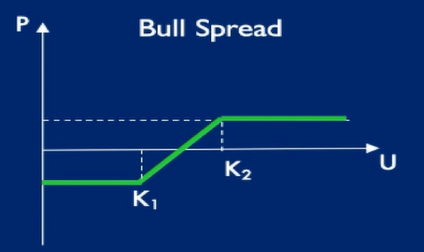
\includegraphics[width=.5\textwidth]{bullSpread.PNG}
    \caption{Pay-Off Diagram for \textit{Bull Spread}.}
    \label{fig_BullSpread}
  \end{figure}

  \begin{figure}[ht!]
    \centering
    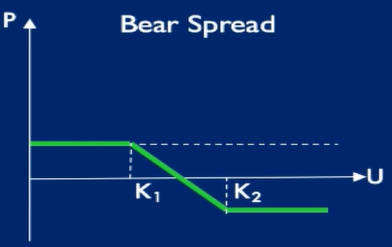
\includegraphics[width=.5\textwidth]{bearSpread.PNG}
    \caption{Pay-Off Diagram for \textit{Bear Spread}.}
    \label{fig_BearSpread}
  \end{figure}

  \begin{figure}[ht!]
    \centering
    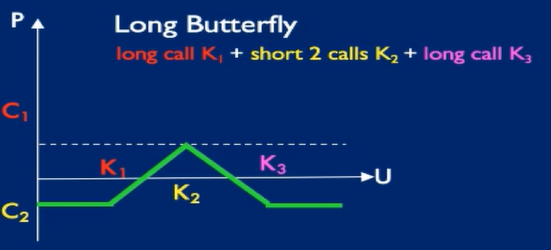
\includegraphics[width=.5\textwidth]{longButterfly.PNG}
    \caption{Pay-Off Diagram for \textit{Long Butterfly}.}
    \label{fig_LongButterfly}
  \end{figure}

  \begin{figure}[ht!]
    \centering
    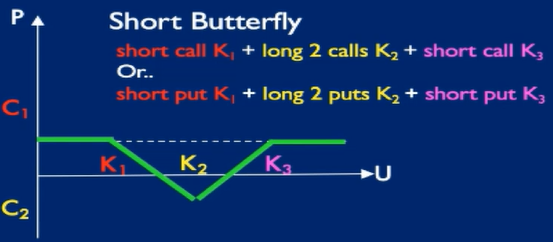
\includegraphics[width=.5\textwidth]{shortButterfly.PNG}
    \caption{Pay-Off Diagram for \textit{Short Butterfly}.}
    \label{fig_ShortButterfly}
  \end{figure}

  \begin{figure}[ht!]
    \centering
    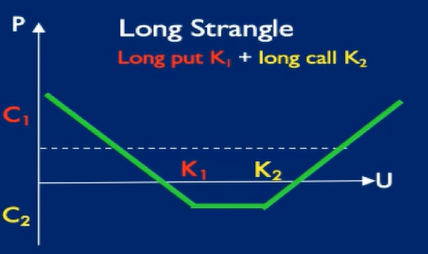
\includegraphics[width=.5\textwidth]{longStrangle.PNG}
    \caption{Pay-Off Diagram for \textit{Long Straddle}.}
    \label{fig_LongStraddle}
  \end{figure}

  \begin{figure}[ht!]
    \centering
    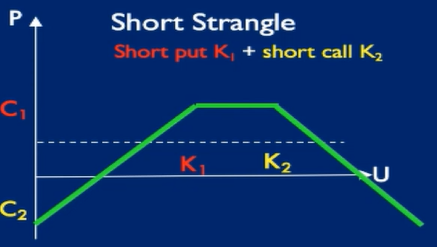
\includegraphics[width=.5\textwidth]{shortStrangle.PNG}
    \caption{Pay-Off Diagram for \textit{Short Straddle}.}
    \label{fig_ShortStraddle}
  \end{figure}

  \begin{figure}[ht!]
    \centering
    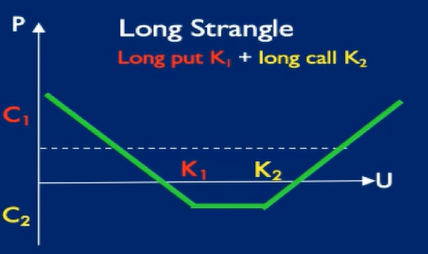
\includegraphics[width=.5\textwidth]{longStrangle.PNG}
    \caption{Pay-Off Diagram for \textit{Long Strangle}.}
    \label{fig_LongStrangle}
  \end{figure}

  \begin{figure}[ht!]
    \centering
    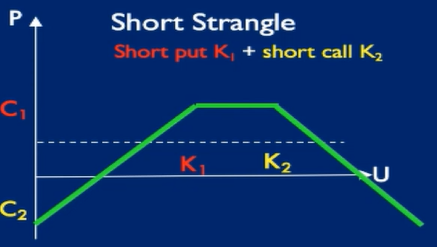
\includegraphics[width=.5\textwidth]{shortStrangle.PNG}
    \caption{Pay-Off Diagram for \textit{Short Strangle}.}
    \label{fig_ShortStrangle}
  \end{figure}

  \begin{figure}[ht!]
    \centering
    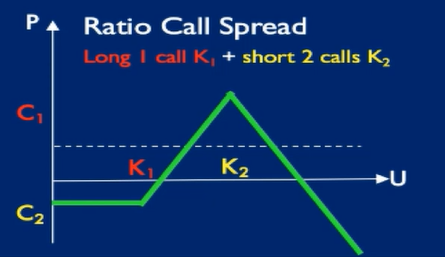
\includegraphics[width=.5\textwidth]{ratioCallSpread.PNG}
    \caption{Pay-Off Diagram for \textit{Ratio Call Spread}.}
    \label{fig_RatioCallSpread}
  \end{figure}

  \begin{figure}[ht!]
    \centering
    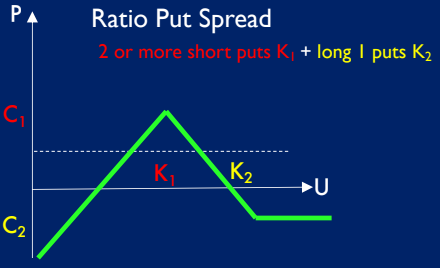
\includegraphics[width=.5\textwidth]{ratioPutSpread.PNG}
    \caption{Pay-Off Diagram for \textit{Ratio Put Spread}.}
    \label{fig_RatioPutSpread}
  \end{figure}

    \begin{figure}[ht!]
      \centering
      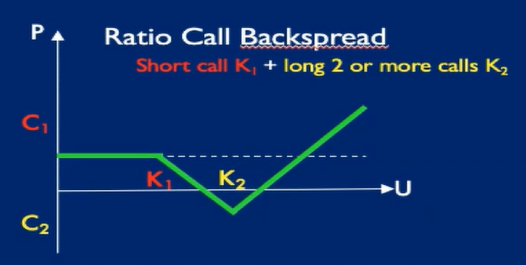
\includegraphics[width=.5\textwidth]{ratioCallBackspread.PNG}
      \caption{Pay-Off Diagram for \textit{Ratio Call Backspread}.}
      \label{fig_RatioCallBackspread}
    \end{figure}

    \begin{figure}[ht!]
      \centering
      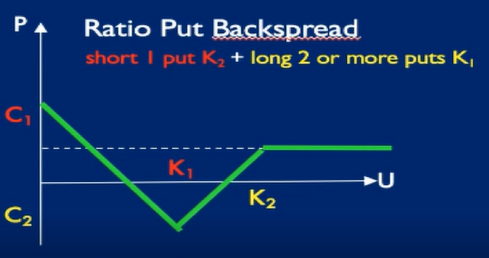
\includegraphics[width=.5\textwidth]{ratioPutBackspread.PNG}
      \caption{Pay-Off Diagram for \textit{Ratio Put Backspread}.}
      \label{fig_RatioPutBackspread}
    \end{figure}

\end{document}
